% Options for packages loaded elsewhere
\PassOptionsToPackage{unicode}{hyperref}
\PassOptionsToPackage{hyphens}{url}
%
\documentclass[
]{book}
\title{Scientific Writing for Health Research}
\author{Ehsan Karim \& Dahn Jeong \& Fardowsa Yusuf}
\date{2022-01-23}

\usepackage{amsmath,amssymb}
\usepackage{lmodern}
\usepackage{iftex}
\ifPDFTeX
  \usepackage[T1]{fontenc}
  \usepackage[utf8]{inputenc}
  \usepackage{textcomp} % provide euro and other symbols
\else % if luatex or xetex
  \usepackage{unicode-math}
  \defaultfontfeatures{Scale=MatchLowercase}
  \defaultfontfeatures[\rmfamily]{Ligatures=TeX,Scale=1}
\fi
% Use upquote if available, for straight quotes in verbatim environments
\IfFileExists{upquote.sty}{\usepackage{upquote}}{}
\IfFileExists{microtype.sty}{% use microtype if available
  \usepackage[]{microtype}
  \UseMicrotypeSet[protrusion]{basicmath} % disable protrusion for tt fonts
}{}
\makeatletter
\@ifundefined{KOMAClassName}{% if non-KOMA class
  \IfFileExists{parskip.sty}{%
    \usepackage{parskip}
  }{% else
    \setlength{\parindent}{0pt}
    \setlength{\parskip}{6pt plus 2pt minus 1pt}}
}{% if KOMA class
  \KOMAoptions{parskip=half}}
\makeatother
\usepackage{xcolor}
\IfFileExists{xurl.sty}{\usepackage{xurl}}{} % add URL line breaks if available
\IfFileExists{bookmark.sty}{\usepackage{bookmark}}{\usepackage{hyperref}}
\hypersetup{
  pdftitle={Scientific Writing for Health Research},
  pdfauthor={Ehsan Karim \& Dahn Jeong \& Fardowsa Yusuf},
  hidelinks,
  pdfcreator={LaTeX via pandoc}}
\urlstyle{same} % disable monospaced font for URLs
\usepackage{longtable,booktabs,array}
\usepackage{calc} % for calculating minipage widths
% Correct order of tables after \paragraph or \subparagraph
\usepackage{etoolbox}
\makeatletter
\patchcmd\longtable{\par}{\if@noskipsec\mbox{}\fi\par}{}{}
\makeatother
% Allow footnotes in longtable head/foot
\IfFileExists{footnotehyper.sty}{\usepackage{footnotehyper}}{\usepackage{footnote}}
\makesavenoteenv{longtable}
\usepackage{graphicx}
\makeatletter
\def\maxwidth{\ifdim\Gin@nat@width>\linewidth\linewidth\else\Gin@nat@width\fi}
\def\maxheight{\ifdim\Gin@nat@height>\textheight\textheight\else\Gin@nat@height\fi}
\makeatother
% Scale images if necessary, so that they will not overflow the page
% margins by default, and it is still possible to overwrite the defaults
% using explicit options in \includegraphics[width, height, ...]{}
\setkeys{Gin}{width=\maxwidth,height=\maxheight,keepaspectratio}
% Set default figure placement to htbp
\makeatletter
\def\fps@figure{htbp}
\makeatother
\setlength{\emergencystretch}{3em} % prevent overfull lines
\providecommand{\tightlist}{%
  \setlength{\itemsep}{0pt}\setlength{\parskip}{0pt}}
\setcounter{secnumdepth}{5}
\newlength{\cslhangindent}
\setlength{\cslhangindent}{1.5em}
\newlength{\csllabelwidth}
\setlength{\csllabelwidth}{3em}
\newlength{\cslentryspacingunit} % times entry-spacing
\setlength{\cslentryspacingunit}{\parskip}
\newenvironment{CSLReferences}[2] % #1 hanging-ident, #2 entry spacing
 {% don't indent paragraphs
  \setlength{\parindent}{0pt}
  % turn on hanging indent if param 1 is 1
  \ifodd #1
  \let\oldpar\par
  \def\par{\hangindent=\cslhangindent\oldpar}
  \fi
  % set entry spacing
  \setlength{\parskip}{#2\cslentryspacingunit}
 }%
 {}
\usepackage{calc}
\newcommand{\CSLBlock}[1]{#1\hfill\break}
\newcommand{\CSLLeftMargin}[1]{\parbox[t]{\csllabelwidth}{#1}}
\newcommand{\CSLRightInline}[1]{\parbox[t]{\linewidth - \csllabelwidth}{#1}\break}
\newcommand{\CSLIndent}[1]{\hspace{\cslhangindent}#1}
\usepackage{booktabs}
\usepackage{amsthm}
\makeatletter
\def\thm@space@setup{%
  \thm@preskip=8pt plus 2pt minus 4pt
  \thm@postskip=\thm@preskip
}
\makeatother
\usepackage{tcolorbox}
\newtcolorbox{blackbox}{colback=black,colframe=orange,coltext=white,boxsep=5pt,arc=4pt}
\usepackage{color}
\usepackage{framed}
\setlength{\fboxsep}{.8em}
\ifLuaTeX
  \usepackage{selnolig}  % disable illegal ligatures
\fi
\usepackage[]{natbib}
\bibliographystyle{apalike}

\begin{document}
\maketitle

{
\setcounter{tocdepth}{1}
\tableofcontents
}
\newenvironment{blackbox}{
  \definecolor{shadecolor}{rgb}{0, 0, 0}  % black
  \color{white}
  \begin{shaded}}
 {\end{shaded}}

\hypertarget{project-summary}{%
\chapter*{Project Summary}\label{project-summary}}
\addcontentsline{toc}{chapter}{Project Summary}

SPPH 504-007 is a required Ph.D.~level UBC credit course for SPPH students. One of the components of this course has a focus on scientific communication. Specifically, communicating with the scientific community about an epidemiological study that has been designed to answer a particular health research question and appropriately interpreting the study results. Students write a research article suitable for submission to an academic peer-reviewed health journal for publication. However, a general challenge of teaching scientific communication is that most of the associated teaching materials and references are either overly general (not discipline-specific, do not take into account applications to healthcare), or not openly accessible (expensive textbooks). Also, SPPH students have varying academic backgrounds, and many are not familiar with new scientific writing collaboration tools that

\begin{enumerate}
\def\labelenumi{(\roman{enumi})}
\tightlist
\item
  are helpful for managing collaborative projects and
\item
  can aid in conducting reproducible research.
\end{enumerate}

This OER project will allow us to make the course content open to other UBC health researchers who struggle with scientific writing and introduce them to tools that will help them manage collaborative group research projects.

The project aims to create and share openly accessible high-quality OER content through a step-by-step educational guide on how to write scientific articles for peer-reviewed journals, with a specific focus on communicating with the health research community. Specific topics include:

\begin{enumerate}
\def\labelenumi{\arabic{enumi}.}
\tightlist
\item
  Scientific writing basics, components of a good research question
\item
  Writing the `Introduction' section, identifying a gap in the literature
\item
  Writing the `Methods' section, describing the data sources/collection, study design, and statistical analysis
\item
  Presenting tables and figures, and writing the `Results' section
\item
  Writing the `Discussion' section, interpreting results, stating the implications, strengths and limitations of the study, and future research
\item
  Introducing tools for managing collaborative scientific writing projects and reproducible research (e.g., RMarkdown, GitHub).
\end{enumerate}

\hypertarget{project-goals}{%
\section*{Project Goals}\label{project-goals}}
\addcontentsline{toc}{section}{Project Goals}

\textbf{Background}: The principal applicant is teaching a UBC course (SPPH 504-007). In this course, one of the components is the communication of scientific research findings through scientific writing. The specific goals are stated below.

\textbf{Goals}: The goals of the project are to (1) create and update course content and materials as open educational resources (OERs), and (2) openly share a step-by-step guide (i.e., written OER content, primarily text) on how to write scientific articles for peer-reviewed journals (in the ``IMRaD'' format; structured in the following sections: Introduction, Methods, Results, and Discussion). (3) Introduce some cutting-edge tools helpful for managing collaborative scientific writing projects and conducting reproducible research (e.g., RMarkdown, GitHub).

\textbf{Implication}: One obvious implication is increased accessibility to students. Currently, the course SPPH 504-007 is restricted to SPPH Ph.D.~students. If this rapid grant project is successful, this content will be openly accessible and will potentially help health researchers across campus interested in publishing manuscripts on their health data research. Examples of people who will directly benefit from this open access project include: SPPH master's students (e.g., MSc, MPH, MHA, who cannot currently register for this course), researchers from all the Departments in the UBC Faculty of Medicine, and any other Departments with researchers that conduct healthcare and biomedical data analysis and research.

\textbf{Format}: Content will primarily be text, that will be placed on an openly accessible GitHub page. Where necessary, tables, pictures and multi-media will be included. Short videos will be embedded to summarize important sections of the content.

\hypertarget{funding}{%
\section*{Funding}\label{funding}}
\addcontentsline{toc}{section}{Funding}

\begin{itemize}
\tightlist
\item
  \href{https://oerfund.open.ubc.ca/oer-rapid-innovation-grants/}{UBC OER Rapid Innovation}
\item
  \href{https://facultystaff.students.ubc.ca/student-engagement/centre-student-involvement-careers/work-learn}{UBC Work Learn}
\end{itemize}

\hypertarget{version-history}{%
\section*{Version history}\label{version-history}}
\addcontentsline{toc}{section}{Version history}

Initial outlines were created for SPPH 504-007 during 2018-2021. In 2021, though OER Fund Rapid Innovation Grant and WorkLearn program, a GRA was hired to convert the outlines to drafts, that were revised and updated by other contributors.

Feel free to \href{https://ehsank.com/}{reach out} for any comments, corrections, suggestions.

\hypertarget{contributor-list}{%
\section*{Contributor list}\label{contributor-list}}
\addcontentsline{toc}{section}{Contributor list}

\begin{longtable}[]{@{}ll@{}}
\toprule
\endhead
Dahn Jeong & SPPH, UBC \\
Fardowsa Yusuf & SPPH, UBC \\
\href{https://ehsank.com/}{Ehsan Karim} & SPPH, UBC \\
\bottomrule
\end{longtable}

\hypertarget{license}{%
\section*{License}\label{license}}
\addcontentsline{toc}{section}{License}


\includegraphics[width=0.25\linewidth]{images/by}

The online version of this book is licensed under the \href{https://creativecommons.org/licenses/by/4.0/}{Attribution 4.0 International (CC BY 4.0)} International License. You may share, and adapt the content.

\begin{rmdcomment}
\textbf{How to cite}

Karim ME, Jeong D, Yusuf F (2021) Scientific Writing for Health
Research. URL:
\url{https://ehsanx.github.io/Scientific-Writing-for-Health-Research/}
\end{rmdcomment}

\hypertarget{research-question}{%
\chapter{Research Question}\label{research-question}}

The first step in conducting a scientific study is to develop a research question; however, this can be a difficult process. Research questions organize and direct the study, communicate the research study's goal to the readers, define the study's boundaries and limitations, and inform researchers on how to conduct the study. A good research question can serve all of these purposes, but developing a ``good'' research question can be difficult and time-consuming. A good research question should address the clinical or population health problem under investigation. Furthermore, the significance of a study's findings is determined by how well it addresses the research question; therefore, not asking the ``right'' research question can jeopardize the validity of the whole study.

Generally, the process of formulating a new research question begins with a public health or clinical problem that needs to be addressed. In health sciences research, the rationale for conducting a research study is typically to address at least one of three issues: the existing evidence is scarce, the current literature contains conflicting evidence, or the evidence base can be improved \citep{fandino2019formulating}. As a result, conducting a thorough literature search on the topic of interest is frequently required in order to formulate a good research question. In addition, the answers to the research question should address an aspect of the specific problem that was identified, and be supportive of the study's rationale. In many instances, this requires narrowing and specifying the research question from a broader, more general question. It has previously been suggested that using a PICOT (population, intervention, comparator, outcome and time frame) framework can help researchers formulate a good research question and can ensure higher quality reporting in studies \citep{thabane2009posing, rios2010association}. A well-structured research question will guide the implementation of the study as well as the reporting of the results. The FINER criteria may also be used to assess the quality of the research question and refine it as needed \citep{thabane2009posing}. In this chapter, we discuss the PICOT framework and FINER criteria for developing a good research question in population and public health research.

\hypertarget{framing-a-research-question-using-the-picot-framework}{%
\section{Framing a research question using the PICOT framework}\label{framing-a-research-question-using-the-picot-framework}}

Formulating and refining the research question using the PICOT framework can inform which study design is most appropriate, what types of data should be collected and what types of analytical methods are most suitable to answer the research question. The framework has many different variations, but the general framework for studies in health research is as follows:

Table 1: Key elements and guiding questions for the PICOT framework

\begin{longtable}[]{@{}
  >{\raggedright\arraybackslash}p{(\columnwidth - 2\tabcolsep) * \real{0.50}}
  >{\raggedright\arraybackslash}p{(\columnwidth - 2\tabcolsep) * \real{0.50}}@{}}
\toprule
\begin{minipage}[b]{\linewidth}\raggedright
Element
\end{minipage} & \begin{minipage}[b]{\linewidth}\raggedright
Description and guiding questions
\end{minipage} \\
\midrule
\endhead
\textbf{P opulation} & \textbf{Specify the target population and study sample} \\
& \emph{What is the target population of the data source?} \\
& \emph{How broad or narrow is the target population?} \\
& \emph{To whom will your research question be generalizable to?} \\
& \emph{Who is included in the study sample that you are trying to make inferences about?} \\
\textbf{I ntervention, treatment or exposure} & \textbf{Specify the intervention, treatment or exposure} \\
& \emph{What is the primary experimental condition that you want to test?} \\
& \emph{What is the intervention / treatment / diagnostic test / procedure?} \\
& \emph{What is the exposure or the explanatory variable of interest?} \\
\textbf{C omparator} & \textbf{Specify the ``control'' group (e.g., standard of care, control, no exposure)} \\
& \emph{Who is included in the comparison group to contrast with the exposed group?} \\
& \emph{What is the standard of care to which the intervention/treatment is compared to?} \\
& \emph{Are there multiple comparison groups?} \\
\textbf{O utcome} & \textbf{Specify the outcome of interest} \\
& \emph{Is the outcome variable objective or subjective?} \\
& \emph{How is the outcome variable measured? Is the outcome quantifiable?} \\
& \emph{Is the measurement tool validated?} \\
& \emph{Is the outcome measurement reproducible? How precise is the measurement?} \\
& \emph{Can temporality be established to avoid the possibility of reverse causality?} \\
& \emph{Are there any secondary outcomes of interest?} \\
\textbf{T ime frame} & \textbf{Specify the time frame in which recruitment, follow-up and data collection will take place} \\
& \emph{When did follow-up happen?} \\
& \emph{When were the measurements taken?} \\
& \emph{How often are the outcomes measured?} \\
\textbf{S etting (optional)} & \textbf{Identify the setting of the study sample to understand the generalizability of findings and provide appropriate interpretations} \\
& \emph{What are the inclusion/exclusion criteria?} \\
\bottomrule
\end{longtable}

\hypertarget{evaluating-research-questions-using-finer-criteria}{%
\section{Evaluating research questions using FINER criteria}\label{evaluating-research-questions-using-finer-criteria}}

Once the research question is developed using the PICOT framework, the FINER criteria can be used to assess the quality of the research question and determine if the research is feasible.

Table 2: Key elements and guiding questions for the FINER criteria

\begin{longtable}[]{@{}
  >{\raggedright\arraybackslash}p{(\columnwidth - 2\tabcolsep) * \real{0.50}}
  >{\raggedright\arraybackslash}p{(\columnwidth - 2\tabcolsep) * \real{0.50}}@{}}
\toprule
\begin{minipage}[b]{\linewidth}\raggedright
Element
\end{minipage} & \begin{minipage}[b]{\linewidth}\raggedright
Description and guiding questions
\end{minipage} \\
\midrule
\endhead
\textbf{F easible?} & \textbf{The feasibility criterion should ensure that the research is doable and the results will be generated in a reasonable time frame} \\
& \emph{Is the research feasible?} \\
& \emph{Is the exposure/treatment or outcome rare?} \\
& \emph{Will it be possible to obtain an adequate sample size?} \\
& \emph{Is the study population representative of the target population?} \\
& \emph{Is there an appropriate study design to address the research question?} \\
& \emph{Is the scope of the study manageable?} \\
\textbf{I nteresting?} & \textbf{This criterion encourages researchers to think about who the target audience of the research study would be} \\
& \emph{Who would be interested in this research?} \\
& \emph{Who is the target audience?} \\
& \emph{Who would be the knowledge users of this research?} \\
& \emph{How will you make it ``interesting'' to the target audience?} \\
\textbf{N ovel?} & \textbf{The research question should generate evidence that adds to the existing literature} \\
& \emph{Is the research original and novel?} \\
& \emph{Is the research question already answered in the literature?} \\
& \emph{What does this research add?} \\
\textbf{E thical?} & \textbf{It is critical to think about the ethical implications of the proposed study} \\
& \emph{How will the research process and dissemination of findings affect the study participants or the target population?} \\
& \emph{Is this research question ethical?} \\
& \emph{Will the findings of the study harm anyone? Create or exacerbate any stigma?} \\
& \emph{Will this study meet the evaluation criteria of the ethics review board?} \\
\textbf{R elevant?} & \textbf{The proposed research should generate knowledge that is relevant to the topic of interest} \\
& \emph{Will answering the research question provide relevant information for the clinical or public health problem identified?} \\
& \emph{How is this research relevant for the topic in question?} \\
& \emph{Will the findings of this study contribute to the existing literature?} \\
& \emph{Does this research address a current need?} \\
& \emph{Would this research generate further investigations in the future?} \\
\bottomrule
\end{longtable}

\hypertarget{tips-for-formulating-a-good-research-question}{%
\section{Tips for formulating a good research question}\label{tips-for-formulating-a-good-research-question}}

A research question needs to be aligned with the data, methods and results. In addition, a good research question should have the following characteristics: clarity, specificity, empirical support, and relevance. Questions in population and public health research typically ask about phenomena related to health and may focus on comparisons, associations, relationships, or descriptions of variables \citep{creswell2017research}. Once you have a broad, general idea of the question you want to investigate, try to describe the goal of the research study as precisely as possible, for example, the gap in knowledge you want to fill or the new evidence you want to generate for a question previously considered in the literature \citep{vandenbroucke2018ideas}. Determining this objective can be helpful when deciding what types of results you need to present. Vandenbroucke and Pearce \citep{vandenbroucke2018ideas} advise describing what table or figure is required to achieve the goal. For example, what table or figure would be needed to fill the knowledge gap. Following this process, the questions will become clearer and guide what types of study design and methods are required to achieve the study objective and attain results.

The most common pitfalls when developing research questions are that the questions incorporate the methods or the study's expected outcomes \citep{mayo2013research}. Furthermore, the clarity of the research question can be impeded by the lack of a clear parameter to assess the relationship or association between exposure and outcome \citep{mayo2013research}.

We propose the following overall roadmap for developing a good research question:

\begin{enumerate}
\def\labelenumi{\arabic{enumi}.}
\tightlist
\item
  Gain an understanding of the research context
\item
  Experiment with a few different PICOT(S) combinations
\item
  Choose the best set of combinations and narrow the research question
\item
  Use the FINER criteria to evaluate the research question's quality
\item
  ``Prune'' the research question by removing any extraneous details \citep{vandenbroucke2018ideas}
\end{enumerate}

A good research question can inform the study objective, data collection, methodology and the relevance of the findings. Not having a good research question can create confusion for readers and reviewers, make the research aimless and the interpretation of the results may be difficult or pointless. Therefore, developing a clear, well-structured research question is a critical step in any scientific investigation.

\hypertarget{statistical-analysis-plans}{%
\section{Statistical analysis plans}\label{statistical-analysis-plans}}

Statistical analysis plans (SAP) are also known as data analysis plans (DAP) or reporting analysis plans (RAP). A statistical analysis plan describes the study variables and the plan for analyzing a data \textbf{before} conducting the analysis; this is essentially the strategy for connecting the study objective to the data analysis that will answer the research question. SAPs have been used in biomedical research and in clinical trials for many years; statistical analysis plans for clinical trials are registered and made publicly available in repositories such as \href{http://www.clinicaltrials.gov/}{ClinicalTrials.gov}. In fact, the National Institutes of Health (NIH) in the United States established policies for reporting NIH-funded clinical trials in 2016, requiring researchers to report full protocol and statistical analysis plan, along with levels of specification for outcome measures, information about adverse events and collection method, and baseline information and characteristics associated with primary outcome measures \citep{zarin2016trial}. Pre-registering SAPs can prevent \emph{``P-value hacking''}, which can occur when researchers \emph{``shop around for a statistical test to give them the P-value that they love''} \citep{yuan2019guide}. By registering pre-specified SAPs, researchers can help improve the study reproducibility and reduce bias \citep{kahan2020public}.

In observational studies, SAPs are much less adopted compared to clinical trials \citep{thor2020registering}; however, the discussion around its use and value have been growing. In this chapter, we discuss the use of SAPs for observational studies, and propose some key components of SAP for observational studies.

\hypertarget{the-value-of-statistical-analysis-plans-in-observational-studies}{%
\subsection{The value of statistical analysis plans in observational studies}\label{the-value-of-statistical-analysis-plans-in-observational-studies}}

Many observational studies are based on large datasets, or ``big data,'' which is defined as heterogeneous datasets linked to a single dataset, with a large number of observations and variables, and that is either real-time or frequently updated \citep{ehrenstein2017clinical}. With these big data and powerful statistical software and methods, finding statistically significant associations without pre-established study objectives, research questions and hypotheses has become easier \citep{yuan2019guide}. These types of analyses can produce statistically significant findings without implications to clinical relevance or justification. SAPs can be useful in ensuring that the analytical methods are planned ahead of time in relation to the research question and objectives, and that this procedure is transparent.

As the findings from observational studies may have an impact on public health policies, guidelines and decision-making, it is critical to ensure that these studies are of high standard, that analyses are pre-specified based on relevance to public health, and that they are replicable. When there is no pre-established SAP specifying the primary outcome variable, outcome reporting bias can occur \citep{cafri2018mitigating}. Many efforts have been made to reduce reporting bias in observational studies, such as STROBE guidelines \citep{von2007strengthening}. The use of SAPs has also been suggested, and that only the variables that researchers pre-specified as variables of interest be made available to them to limit post hoc analyses \citep{thomas2012value, williams2010registration}. Some even argue that SAPs should be required even before obtaining data, during the application stage of data access \citep{trinh2013statistical, hiemstra2019debate}. In fact, to obtain access to big data, it is often required to submit a data request form that contains some key elements of a SAP \citep{dars2021, popdata2021}.

SAPs also have an important role in identifying potential biases, such as selection bias (based on the inclusion/exclusion criteria) or measurement bias, and can help researchers plan how to minimize and address these biases.

\hypertarget{guide-on-writing-an-sap-for-observational-studies}{%
\subsection{Guide on writing an SAP for observational studies}\label{guide-on-writing-an-sap-for-observational-studies}}

Based on the guidelines for SAP for clinical trials \citep{gamble2017guidelines} and literature suggesting its' adaptation for observational studies \citep{yuan2019guide, thomas2012value, hiemstra2019debate}, we suggest the following four key components for writing SAP for observational studies in health sciences research:

\begin{itemize}
\item
  \textbf{Study objectives and hypotheses}

  \begin{itemize}
  \tightlist
  \item
    Broad research area, study background and rationale
  \item
    Research question (e.g.~using PICOT framework and FINER criteria)
  \item
    Hypothesis and aims
  \end{itemize}
\item
  \textbf{Study population}

  \begin{itemize}
  \tightlist
  \item
    Study design (e.g.~cross-sectional, prospective cohort)
  \item
    Study sample and inclusion/exclusion criteria
  \item
    Study period (time points under consideration in the data source)
  \item
    Baseline characteristics of study population
  \end{itemize}
\item
  \textbf{Study variables: definitions, types, how they are measured}

  \begin{itemize}
  \tightlist
  \item
    Outcome variables
  \item
    Explanatory/exposure variables
  \item
    Covariates (e.g.~mediators, colliders, confounders)
  \item
    Derived variables
  \end{itemize}
\item
  \textbf{Statistical analysis methods}

  \begin{itemize}
  \tightlist
  \item
    Defined level for statistical significance
  \item
    Plans for handling missing data, correlation, bias and confounding, and repetitive analyses
  \item
    Details on model building and variable selection
  \item
    Details on additional methods if model assumptions do not hold (e.g.~normality, proportional hazards)
  \item
    Strategies for interaction or subgroup analysis and sensitivity analyses
  \end{itemize}
\end{itemize}

Finally, SAPs can be useful in observational studies because they encourage detailed and rigorous planning of the study rather than disorganized and spontaneous data analysis. They can also optimize the resources to focus on the right methods for the research questions, and ensure methodological transparency and replicability of findings. We propose the following two broad questions that can be used to determine whether the SAP is appropriate:

\begin{enumerate}
\def\labelenumi{\arabic{enumi}.}
\tightlist
\item
  Does the SAP help in answering the research question or achieving the original study objective?
\item
  Are the planned analyses appropriate in the context of the research question?
\end{enumerate}

\hypertarget{introduction-section}{%
\chapter{Introduction Section}\label{introduction-section}}

A scientific research paper generally follows the format of IMRaD (Introduction, Methods, Results and Discussion). The introduction section sets the stage for the entire paper and introduces the topic of interest to the audience. This first section provides a broad context of the issue under investigation, summarizes what is known and unknown, and tries to convince the readers that this particular study will be a valuable addition to current knowledge.

There are several guidelines suggesting how to best structure the introduction section for a research paper \citep[p.84-88]{cals2013effective, bahadoran2018principles, heard2016scientist}. Typically, a well-written introduction section will contain broader background information on the topic, a summary of key existing knowledge relevant to the specific problem, the gap in the current knowledge (rationale), and the research question and/or the hypothesis. Though not essential, some authors may opt to briefly describe the study design and methods.

\hypertarget{funnel-shape}{%
\section{Funnel shape}\label{funnel-shape}}

To better organize the main components of the introduction, it may be useful to build an outline or a skeleton of the section. One approach could be adopting a ``funnel shape'' or an inverted pyramid shape to organize the components. Based on the funnel shape, the introduction section has five key elements going from broad to narrow: big picture, what is known, what is unknown, research question and methods/design (see Figure 1).

\begin{figure}

{\centering 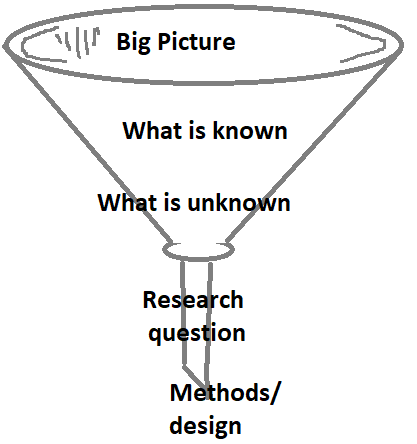
\includegraphics[width=0.25\linewidth]{images/funnel} 

}

\caption{The typical funnel shape of an Introduction section.}\label{fig:funnel}
\end{figure}

\begin{enumerate}
\def\labelenumi{\arabic{enumi}.}
\item
  \textbf{Big picture}: the introduction starts with the big picture, represented by the broad opening of the funnel shape. The big picture introduces the general context of the research area and provides an overview of ``why this topic or issue is important.'' For a research paper in population and public health, it is a good idea to present the broader background information on the health-related topic. This may include the magnitude of the problem and/or the burden of disease (e.g., incidence, prevalence or cost). The big picture should provide the audience with an understanding of the study outcome or explanatory variable from a public health perspective.
\item
  \textbf{What is known}: from the big picture, the author narrows down to a more specific research area under investigation. This part should outline the existing knowledge of the research area by providing a summary of the evidence, including the landmark and recent studies. This summary should cite the most current and comprehensive knowledge on the subject. Remember that the evidence cited should be directly relevant to your specific study and inform your research question. These summaries should focus on the particular exposure or disease of interest (e.g., intervention or outcome elements of the PICOT framework) \citep{thabane2009posing}.
\item
  \textbf{What is unknown}: as the funnel further narrows, this part should present a synthesis of the reasons why the issue is important (in the big picture), what is already known, and what is unknown, to convince the audience that there is a need to conduct your specific study. This part can include the gaps in current knowledge, any inconsistencies in the literature, gaps in the methodology or the need for different or better methodology. When describing what is unknown, the author should highlight the importance of conducting the present study and persuade the readers that this analysis was needed (rationale). Who would likely benefit from this study should also be highlighted. For example, if there is a previous study that answered the same research question, a clear and compelling argument on the need for the updated study should be included.
\item
  \textbf{Research question}: following the identification of the gap in current knowledge, this part outlines the specific purpose of the study. It should include the study objective and/or hypothesis that will address the identified gap in current knowledge.
\item
  \textbf{Methods/design}: as the last stage of the funnel, this part can briefly introduce the approach used to answer the research question. This can include the study design or methods, however, a brief summary is sufficient as the methodological approach will be described in depth in the methods section.
\end{enumerate}

\hypertarget{examples}{%
\section{Examples}\label{examples}}

\hypertarget{example-1}{%
\subsection{Example 1}\label{example-1}}

The first example is taken from \citet{nisingizwe2020perceived}. You can download the open access PDF from \href{https://bmcpregnancychildbirth.biomedcentral.com/track/pdf/10.1186/s12884-020-2775-8.pdf}{here}.

Table 1: A study about the association between perceived barriers to health care access and inadequate antenatal care visits \citep{nisingizwe2020perceived}

\begin{longtable}[]{@{}
  >{\raggedright\arraybackslash}p{(\columnwidth - 4\tabcolsep) * \real{0.15}}
  >{\centering\arraybackslash}p{(\columnwidth - 4\tabcolsep) * \real{0.25}}
  >{\raggedright\arraybackslash}p{(\columnwidth - 4\tabcolsep) * \real{0.60}}@{}}
\toprule
\begin{minipage}[b]{\linewidth}\raggedright
Elements
\end{minipage} & \begin{minipage}[b]{\linewidth}\centering
Location in the introduction section
\end{minipage} & \begin{minipage}[b]{\linewidth}\raggedright
Comments
\end{minipage} \\
\midrule
\endhead
Big picture & 1st paragraph (\emph{``Maternal and neonatal mortality \ldots{}''}) & Authors introduce the public health problem of interest, maternal and neonatal mortality, by presenting the magnitude of the problem and the burden of disease. This paragraph highlights the importance of the public health problem. \\
What is known & 2nd paragraph (\emph{``Timely and frequency of ANC \ldots{}''}) & The authors describe the more specific research area: the relationship between receiving adequate antenatal care (ANC) and barriers to healthcare. \\
& 3rd paragraph (\emph{``However, the country' maternal and neonatal death rates \ldots{}''}) & The authors provide a summary of the existing knowledge relevant to the study that informs the research question. \\
What is unknown & 4th paragraph (\emph{``To date, there is a paucity \ldots{}''}) & The authors present what is unknown: the relationship between perceived barriers to health care and inadequate ANC visits in Rwanda. In addition, they identify previous studies and the gaps in the current knowledge. The clear identification of a research gap supports the stated rationale for conducting this particular study. \\
Research question & 4th paragraph (\emph{``Therefore, this study aims \ldots{}''}) & Following the identification of the gap in current knowledge, the authors present the specific purpose of the study. \\
& 5th paragraph (\emph{``We hypothesized that \ldots{}''}) & The authors present the hypothesis for the research question. \\
& 5th paragraph (\emph{``This study will contribute to \ldots{}''}) & the authors include a brief summary of the key study implications to convince the audience that this research paper will add value to the field of study. \\
Methods/design & & The authors have not included a specific section summarizing the methodological approach used in the study to answer the research question. However, in the 4th paragraph, they indicated that the study will use a ``country representative sample'' from ``2015 DHS data''. \\
\bottomrule
\end{longtable}

\hypertarget{example-2}{%
\subsection{Example 2}\label{example-2}}

The second example is taken from \citet{basham2019multimorbidity}. You can download the open access PDF from \href{https://www.tandfonline.com/doi/epub/10.1080/22423982.2019.1607703}{here}.

Table 1: A study about prevalence of multimorbidity in northern vs.~southern Canada \citep{basham2019multimorbidity}

\begin{longtable}[]{@{}
  >{\raggedright\arraybackslash}p{(\columnwidth - 4\tabcolsep) * \real{0.15}}
  >{\centering\arraybackslash}p{(\columnwidth - 4\tabcolsep) * \real{0.25}}
  >{\raggedright\arraybackslash}p{(\columnwidth - 4\tabcolsep) * \real{0.60}}@{}}
\toprule
\begin{minipage}[b]{\linewidth}\raggedright
Elements
\end{minipage} & \begin{minipage}[b]{\linewidth}\centering
Location in the introduction section
\end{minipage} & \begin{minipage}[b]{\linewidth}\raggedright
Comments
\end{minipage} \\
\midrule
\endhead
Big picture & 1st paragraph (\emph{``Multimorbidity is common among \ldots{}''}) & The public health problem of interest, multimorbidity, is introduced along with the magnitude of the problem and the burden of disease. \\
What is known and unknown & 2nd paragraph (\emph{``Northern Canada, which \ldots{}''}) and 3rd paragraph (\emph{``The equivocacy of findings \ldots{}''}) & The more specific research area, multimorbidity in Canadian provinces and territories, is contextualized. The authors provide a summary of relevant previous studies and highlight the gaps within these studies. The synthesis of the ``big picture,'' ``what is known'' and ``what is unknown'' elements supports the rationale for this particular study. \\
& & \\
Research question & 3rd paragraph (\emph{``The primary aim of this study \ldots{}''}) & Once the need for this particular study is identified, the authors present the specific research question and the hypothesis. \\
Methods/design & 3rd paragraph (\emph{``This study describes multimorbidity \ldots{}''}) & The authors briefly mention the methodological approach used in the study. \\
\bottomrule
\end{longtable}

Through these 2 examples, we have looked at the key elements of an introduction section of a scientific article in population and public health research. The introduction section provides the general context of the topic (big picture), the narrower research area and what is known, the gap in the existing knowledge, the specific purpose of the study and a summary of the methods and design.

\hypertarget{importance-of-a-hook}{%
\subsection{Importance of a `hook'}\label{importance-of-a-hook}}

As the author and researcher, you have the knowledge of the ``whole story'' of your study from start to end. Hence, you can write the introduction strategically. The introduction section introduces the public health problem to the audience and tries to capture their interest to continue reading. In a newspaper or magazine article, the writer aims to grab the readers' attention with a ``hook'' at the beginning. In a scientific article, although you don't necessarily want to give out all the findings and study implications initially, you should utilize the introduction section to incite the readers' and reviewers' interest. By clearly outlining the key components, the introduction section should convince the audience that the population/public health issue under investigation is critical to address and that your particular study is novel and valuable.

\hypertarget{common-pitfalls}{%
\section{Common pitfalls}\label{common-pitfalls}}

\begin{itemize}
\tightlist
\item
  Common pitfalls in the introduction section include \emph{incomplete, inaccurate or outdated reviews of the literature} on the topic. For example, including literature that is tangentially related or within the same field but not directly related to the problem, may result in an incomplete or confusing review of the background knowledge. Including inadequate, incomplete or outdated information may result in the rejection of the paper.
\item
  Not adequately explaining the \emph{importance or the relevance of the current knowledge in relation to the study aims} is another pitfall. This can lead to an introduction section that is less effective in communicating the relevancy and novelty of your study.
\end{itemize}

\hypertarget{tips}{%
\section{Tips}\label{tips}}

\begin{enumerate}
\def\labelenumi{\arabic{enumi}.}
\tightlist
\item
  Arguably, incorporating \emph{clear study aim(s)} and \emph{rationales for the study objectives} are the most important aspects of the introduction section. (i) Aims should be clearly articulated, and the design of the study should be planned accordingly. (ii) Take time to think about the justification of the current study.
\item
  Provide only the \emph{key references} that are needed to describe the background knowledge, as well as what is known and unknown about the topic of interest. Including an excessive amount of literature in the introduction can be distracting. Be mindful that you will have an opportunity to contextualize your research in the literature by comparing your findings with other studies in the Discussion section. The introduction should be focused on setting the tone for what is coming next.
\item
  A lengthy introduction can also make the readers lose interest. A general suggestion is that the introduction section should be about 10-15\% of the whole paper \citep{cals2013effective}.
\item
  If you already have a general idea of the journals that you would like to submit your article to, the introduction can be tailored to the audience of the target journal. For example, if you are interested in submitting to journals with a heavier focus on methodology or epidemiology, you may want to highlight the novelties in the design or methods. If you are interested in submitting to clinician-focused or subject-specific journals, you may emphasize the clinical or public health implications of the study.
\end{enumerate}

\hypertarget{methods-section}{%
\chapter{Methods Section}\label{methods-section}}

Based on the IMRaD (Introduction, Methods, Results and Discussion) format discussed previously, the second section of a scientific research paper is the methods. The purpose of the methods section is to provide a comprehensive picture of the methodological approach of the study in a straightforward and transparent manner. Broadly, the methods section should allow the readers to understand the dataset under consideration and the analytical steps undertaken in the study, and give a sense of reproducibility of the study \citep{annesley2010and, kotz2013effective3}.

\hypertarget{the-bridge}{%
\section{The ``Bridge''}\label{the-bridge}}

Following the introduction section, the methods section connects the previously developed research question to the results section and equips the readers with all methodological details necessary to interpret the findings that will be presented in the next section. As such, the methods section is the ``bridge'' between the introduction and the results section. Typically, the main elements of a methods section are: study design and data collection; setting, analytic sample and variables; data and statistical analysis.

Furthermore, breaking the methods section into sub-sections can be a helpful way to present the methodological approach in an organized fashion. The main elements of the methods section can be presented as sub-sections.

\begin{enumerate}
\def\labelenumi{\arabic{enumi}.}
\item
  \textbf{Statement of study design and data collection:} the study design (e.g.~cohort study, cross-sectional study, etc) and other key elements of the study design should be mentioned early in the methods. The data source(s) and how data was collected should be detailed.

  \begin{enumerate}
  \def\labelenumii{\alph{enumii}.}
  \tightlist
  \item
    Sampling strategy: for cross-sectional studies, it is recommended to describe the sampling design for the data source.
  \end{enumerate}
\item
  \textbf{Setting, analytic sample and variables:} if relevant, the setting, locations and timeframe (e.g.~recruitment, follow-up, data collection) can be described. For the analytic sample, how it was obtained from the target population should be clearly described, including inclusion and exclusion criteria. The key outcome and explanatory variables should be defined, including case definitions or algorithms. You can also present the details of methods of measurement or assessment if they are relevant, or if they are derived from other variables or measures. It is important to identify which covariates were included and why they were included or not included (variable selection).

  \begin{enumerate}
  \def\labelenumii{\alph{enumii}.}
  \item
    For the study population, if there are any differences between people who were included in the study population compared to those who were excluded from the source population, these differences should be described.
  \item
    Ethics approval: a statement about ethics approval from a research ethics board or other ethical considerations should be included.
  \end{enumerate}
\item
  \textbf{Data/statistical analysis:} all statistical methods used for descriptive and inferential analyses should be described, including the methods used to control for confounding. If you have conducted sensitivity analyses, these should be described. The methods section should contain descriptions of statistical approach used for all findings presented in the results section. In general, the statistical program or software and the packages used are also stated in this section.
\end{enumerate}

When writing a scientific paper in epidemiology or in population and public health, the STROBE checklist \citep{von2007strengthening} can be a helpful tool to ensure that you are reporting all necessary components in the methods section. Below we will have a look at two examples of papers presenting survey-based analysis with the STROBE checklist.

\hypertarget{examples-1}{%
\section{Examples}\label{examples-1}}

\hypertarget{example-1-1}{%
\subsection{Example 1}\label{example-1-1}}

This example is taken from \citet{nikiforuk2021influence}, which was based on the NHANES data. You can download the open access PDF from \href{https://www.ncbi.nlm.nih.gov/pmc/articles/PMC8278694/pdf/12889_2021_Article_11267.pdf}{here}.

Table 1: A study about chronic hepatitis C infection and monocyte-to-platelet ratio \citep{nikiforuk2021influence}

\begin{longtable}[]{@{}
  >{\raggedright\arraybackslash}p{(\columnwidth - 4\tabcolsep) * \real{0.15}}
  >{\centering\arraybackslash}p{(\columnwidth - 4\tabcolsep) * \real{0.25}}
  >{\raggedright\arraybackslash}p{(\columnwidth - 4\tabcolsep) * \real{0.60}}@{}}
\toprule
\begin{minipage}[b]{\linewidth}\raggedright
Elements
\end{minipage} & \begin{minipage}[b]{\linewidth}\centering
Location in the methods section
\end{minipage} & \begin{minipage}[b]{\linewidth}\raggedright
Comments
\end{minipage} \\
\midrule
\endhead
Study design & The sub-section titled ``data, design and study population'' & The authors outline briefly this was a cross-sectional study. \\
Setting & The sub-section titled ``data, design and study population'' & The data source for the study, NHANES, is described including the target population, location, timeframe and sampling design. \\
Participants & The second paragraph of the sub-section titled ``analytic sample and variable selection'' & The authors describe how the analytic dataset was created from the data source. Exclusion criteria is also included. Figure 1 in the paper illustrates who were excluded at each stage and helps readers to understand potential sources of selection bias and how these might affect the generalizability. \\
Variables & The first and second paragraphs of the sub-section titled ``analytic sample and variable selection'' & The exposure and outcome variables of interest are clearly defined, including the explanation of how the outcome variable ``monocyte-to-platelet ratio'' was derived from two variables, complete blood count measures of monocyte count and platelet count. The authors include an additional file for more detailed description. The authors also provide the justification of how covariates were identified, with a directed acyclic graph included as an additional file. \\
Data sources/measurement & The sub-sections titled ``analytic sample and variable selection'' & The authors provide information on how the key variables were measured, and further provide a reference for additional information on the data source, NHANES. \\
Bias & Throughout the sub-section titled ``statistical analysis'' & The authors described all methods applied to adjust for any potential confounding, such as in the sub-section ``transformation of the monocyte-to-platelet ratio'' and other methods including missing data and propensity score analyses. \\
Study size & Figure 1 & Figure 1 clearly presents all people who were excluded at each stage and the remaining study sample size. \\
Quantitative variables & The sub-sections titled ``analytic sample and variable selection'' and ``statistical analysis'' & The authors describe how the continuous variables were derived for the outcome variable, and further, how the resulting outcome variable was dichotomized. \\
Statistical methods & Throughout the sub-section titled ``statistical analysis'' & The authors provide adequate information about descriptive, inferential, missing data and sensitivity analyses, including the statistical software and packages. The level of information provided ensures the reproducibility of the results if needed. The authors also include citations for relevant methods or analyses. \\
\bottomrule
\end{longtable}

\hypertarget{example-2-1}{%
\subsection{Example 2}\label{example-2-1}}

This example is taken from \citet{nethery2019household}, which was based on the CCHS data. You can download the open access PDF from \href{https://www.cmajopen.ca/content/cmajo/7/4/E646.full.pdf}{here}.

Table 2: A study about the household income and contraceptive methods \citep{nethery2019household}

\begin{longtable}[]{@{}
  >{\raggedright\arraybackslash}p{(\columnwidth - 4\tabcolsep) * \real{0.15}}
  >{\centering\arraybackslash}p{(\columnwidth - 4\tabcolsep) * \real{0.25}}
  >{\raggedright\arraybackslash}p{(\columnwidth - 4\tabcolsep) * \real{0.60}}@{}}
\toprule
\begin{minipage}[b]{\linewidth}\raggedright
Elements
\end{minipage} & \begin{minipage}[b]{\linewidth}\centering
Location in the methods section
\end{minipage} & \begin{minipage}[b]{\linewidth}\raggedright
Comments
\end{minipage} \\
\midrule
\endhead
Study design & The sub-section titled ``data source, design and study population'' & The authors state that this was a cross-sectional study. \\
Setting & The sub-section titled ``data source, design and study population'' & The data source for the study, CCHS, is described including the target population, location, timeframe, response rates and sampling design. \\
Participants & The sub-section titled ``analytic sample'' & The authors describe how the analytic dataset was drawn from the CCHS data including the inclusion and exclusion criteria. As in the first example, the authors include a flowchart as Figure 1 to illustrate who were included/excluded at each stage, resulting in the analytic sample. \\
Variables & The sub-sections titled ``outcome variables'' and ``exposure variable'' & The definitions of outcome and exposure variables are stated clearly. The authors provide additional details on the outcome variables, including some potential sources of bias, which enhances the readers ability to interpret the findings. The authors also explain how the exposure variable was dichotomized. \\
Data sources/measurement & The sub-sections titled ``outcome variables'' and ``exposure variable'' & The authors outline specific questions from the CCHS (data source) that were used to derive the outcome and exposure variables. \\
Bias & The sub-sections titled ``statistical analysis'' and ``sensitivity analysis'' & The authors describe some of the methods that were used to mitigate potential confounding (e.g.~use of survey weights, multiple imputation, sensitivity analyses). The authors also provide the explanation behind the selection of confounders, providing background references. \\
Study size & Figure 1 & As in the first example, Figure 1 presents all people who were excluded at each stage and the remaining analytic sample size. \\
Quantitative variables & N/A & The key outcome and explanatory variables in this study were binary. In the ``statistical analysis'' sub-section, it is mentioned that the ``age'' variable is included as a confounder, and it isn't clear whether this was a continuous or a categorical variable. However, this is neither key outcome nor explanatory variable, so the level of detail is perhaps not required. \\
Statistical methods & The sub-sections titled ``statistical analysis'' and ``sensitivity analysis'' & The authors provide details on the descriptive, inferential, missing data and sensitivity analyses, including the statistical software and packages. \\
Other & The sub-section titled ``ethics approval'' & The ethics approval for the use of data source is stated briefly. \\
\bottomrule
\end{longtable}

\hypertarget{significance-of-the-methods-section-in-population-and-public-health-research-paper}{%
\section{Significance of the methods section in population and public health research paper}\label{significance-of-the-methods-section-in-population-and-public-health-research-paper}}

In population and public health, the methods section of the research paper should enable readers to assess the internal and external validity of the study. It should provide all the necessary information to understand in which ways the authors have made efforts to try to address their research question as accurately as possible. As Rothman et al.~describes, generally the goal of epidemiologic research is to ``obtain a valid and precise estimate of the frequency of a disease or of the effect of an exposure on the occurrence of a disease in the source population of the study'' \citep[p.128--47]{rothman2008validity}. In addition, as the introduction section would have described the importance of the research question in relation to the population and public health, researchers often aim to generalize the study findings to the relevant population groups. By providing clear and adequate information about the target population and how the study sample was selected from the source population, the methods section allows the readers to assess the generalizability of the study findings.

As such, a well-written methods section in a research paper in population and public health should contain necessary information about the analytical steps undertaken in the study, and sufficient description of the study design and target population to enable readers to understand what some of the potential sources of bias in the study are, and what measures were taken to minimize the bias. This allows the readers to interpret the internal and external validity of the study. A well-written methods section provides credibility and validity of the results and conclusions of the study.

After reading the methods section, the readers should have an understanding of the dataset which is under consideration in the study, who the target population was, how the data was collected, and how the analytic data was created (who are included and excluded). Based on the analytic steps described in the methods section, the readers should also be able to understand how the results and conclusions in the next sections of the paper derive from the statistical analyses. Finally, the readers should be able to replicate the study if needed and reproduce the results if they had access to the data source.

\hypertarget{common-pitfalls-1}{%
\section{Common pitfalls}\label{common-pitfalls-1}}

\begin{itemize}
\tightlist
\item
  Common pitfalls in the methods section can largely arise from not reviewing the key elements of the methods section carefully and missing some of the elements in consequence.
\item
  Missing crucial elements providing information on the potential sources of selection or information bias can result in losing the reviewers' and editors' confidence in the validity and credibility of the study findings.
\item
  Another common problem is not providing any explanations regarding the variable selection (i.e.~how the covariates were included or not included in the model).\\
\item
  Be mindful about plagiarism and self-plagiarism, especially if you are using the same data source or similar methods from previously published work.
\end{itemize}

\hypertarget{tips-1}{%
\section{Tips}\label{tips-1}}

\begin{enumerate}
\def\labelenumi{\arabic{enumi}.}
\tightlist
\item
  As in the introduction section, excessive and unnecessary details are discouraged. Unless the focus of your paper is the methodological approach, only discuss enough details to enable reproducibility and to highlight the elements that are relevant for the interpretation of the results. We talked about presenting the research as a ``story'', any detail that are unnecessary or redundant to understanding this story should be avoided.
\item
  The methods section should also include a statement on the ethical approval or any other ethical considerations.
\item
  It's often a good idea to include a citation for the statistical test or method, if this is relatively unknown to the readers. This can also increase the credibility of the methods presented.
\item
  Some journals focused on patient-oriented research encourage researchers to include any processes or efforts that were made to include patients or the community members during research. If patients or community members were involved in the study at any step, it can be a good idea to describe what their involvement was.
\end{enumerate}

\hypertarget{tables-and-figures}{%
\chapter{Tables and Figures}\label{tables-and-figures}}

So far, we have looked at the components of the introduction and the methods sections of a scientific research paper. Before looking at all the components of the results section, we will discuss the most crucial elements of the results section, and perhaps of the entire research paper, the tables and figures. Tables and figures are an integral part of a scientific article as they give an overview of the results obtained from the analyses. For many readers, reviewers and editors, these are the first elements they will look at when reading a paper. Therefore, well designed tables and figures are an effective tool to convey findings and can make a great impression on the readers even before they dive into the paper.

It is widely known that tables and figures are an efficient way to present the key study findings \citep{kotz2013effective4}. Kotz and Cals \citep{kotz2013effective4} suggest planning on which findings to portray in the tables and figures early in the writing process. Once this is determined, the most important aspect when designing the tables and figures is that they should be `standalone', or self-explanatory. The readers should gain a complete understanding of the message you are trying to convey just by looking at the table or the figure. To help with this, there are a few recommended guidelines for designing tables and figures.

Below we discuss the components that can optimize the tables and figures in a scientific research article in the field of population and public health.

\hypertarget{designing-a-table}{%
\section{Designing a table}\label{designing-a-table}}

As discussed, tables in a scientific paper should be concise, but standalone. Tables must be accompanied with an informative title, descriptive column headers and descriptive row labels. A footnote should also be included that explains any abbreviations used and the analyses that were applied to produce the results in the table.

\begin{itemize}
\tightlist
\item
  \textbf{Titles:} titles should be self-contained and informative. According to the American Journal of Epidemiology, titles should include details on the location of the study, the time period over which the study was conducted and the study population \citep{aje2021instructions}. Even if including these details lengthens the title, it is important to include all the necessary information so that readers don't have to go back to the manuscript to find the information they need to understand the table.
\item
  \textbf{Column headers:} column headers should be succinct but descriptive as these introduce the table to the readers, along with the title.
\item
  \textbf{Row labels:} when variables have multiple categories consider using a hierarchical representation (i.e., via indenting) and specify which category was used as the reference.
\item
  \textbf{Footnote:} footnotes should include the definitions of the abbreviations and details on the statistical tests and analyses used.
\end{itemize}

Furthermore, rather than duplicating information in the main text, the tables should be used to complement it, and vice versa.

You should try to organize the tables in a way that ensures the reader can easily and quickly digest and comprehend the information within. Some formatting tips include:

\begin{itemize}
\tightlist
\item
  Designing the table layout with three horizontal lines in total: a line at the top of the table, a line below the column headers and a line at the bottom of the table. If the table is particularly large, shading can be used to demarcate the rows. Drawing horizontal and vertical lines inside the table is highly discouraged.
\item
  The number of columns should be kept to a minimum. For example, instead of having a column for the p-values, you should consider using significance codes to indicate the level of statistical significance. For example, different numbers of asterisks can be used (*P\textless0.05, **P\textless0.01, ***P\textless0.001) \citep{kotz2013effective4}.
\item
  Whether the p-values are one-sided or two-sided should be specified. Some journals suggest only reporting two-sided p-values unless a one-sided test is required by the study design. As for decimal places for the p-values, the NEJM recommends reporting p-values larger than 0.01 with two decimal places, those between 0.01 and 0.001 with three decimal places, and those smaller than 0.001 as P\textless0.001 \citep{nejm2021author}.
\item
  When reporting p-values or confidence intervals, the statistical test used to obtain the values needs to be described.
\item
  For decimal points, do not report numbers with too many decimal places.
\item
  The units of measurement for the study variables should be reported. For example, age in years or increments of 10 years, BMI in kg/m2, physical activity (min/day), etc.
\item
  When displaying data in a table, do not include too many significant figures.
\item
  Do not over-stylize the data using the bold, italic, and underline options \citep{franzblau2012graphs}.
\end{itemize}

\hypertarget{designing-a-figure}{%
\section{Designing a figure}\label{designing-a-figure}}

A figure can be useful when you have a lot of data that you'd like to describe or when you'd like to convey a key message. Deciding between a table or a figure depends on what kind of information you're looking to present. If your data is representing a trend, pattern or association (in particular, if there is a non-linear trend), a figure may be able to convey the information more efficiently than a table. However, if it is important to present the exact numbers for the results, consider using a table rather than a figure.

Similar to the tables, figures must be accompanied with a detailed title, descriptive labels for the y- and x-axes, a legend explaining any symbols, colours and line types, and a footnote. Generally, the title for a figure generally is placed under the image, and the footnote is placed under the title.

Keep in mind the main message you are aiming to convey with the figure. It can take some time to design a figure that meets your needs. Some general guidelines include:

\begin{itemize}
\item
  Some journals may charge additional fees to print coloured figures. Therefore, it will be likely be less costly to design the initial figure in black and white.
\item
  If you decide to make figures with colours, you should consider colour combinations and palettes that are accessible or colour-blind friendly. For example, the R `ggplot2' package offers some colour-blind friendly palettes \citep{chang}. You can access the chapter \href{http://www.cookbook-r.com/Graphs/Colors_(ggplot2)/\#a-colorblind-friendly-palette}{here}.
\item
  Avoid using unnecessary grid lines inside the graph or plot, except for a reference line when necessary (e.g., a line indicating a Hazard Ratio (HR) or Odds Ratio (OR) of 1.0 in a forest plot).
\item
  When placing graphs and plots side-by-side, be mindful of the scale of the graphs to avoid misleading the readers. It's always a good idea to use the same scale across the graphs and figures.
\item
  Avoid complicated, confusing figures such as 3-dimensional graphs \citep{franzblau2012graphs}.
\end{itemize}

\hypertarget{tables-and-figures-in-population-and-public-health-research-papers}{%
\section{Tables and figures in population and public health research papers}\label{tables-and-figures-in-population-and-public-health-research-papers}}

In research articles in epidemiology or in population and public health, generally, table 1 presents the sociodemographic and/or clinical characteristics of the study population stratified by the levels of the explanatory variable. For research papers based on a large survey datasets, table 1 includes descriptive statistics such as counts (number of people in the study sample in each category), proportions (accounting for the survey design), as well as means and standard deviations (also accounting for the survey design). Table 1 allows readers to compare the variables of interest across the levels of the explanatory/exposure variable of interest and may help them to gain an understanding of the research question. Sometimes, the authors test for differences and include a column for the p-values to indicate whether the variables presented are distributed differentially across the levels of the exposure.

Table 2 usually presents the results of the primary inferential analysis assessing the research question, i.e., the association between the main explanatory and outcome variables under investigation. If there are multiple models used or additional outcomes considered, multiple columns can be included in this table. The footnote for the table usually includes information on the analytical model, the variable selection approach and the relevant tests of significance. This table generally reports the effect of the exposure or the specific level of the explanatory variable on the outcome after adjustment for potential confounders.

Additional tables can be included that present the results of the effect modification analyses or any other sensitivity analyses that provide additional clarity to the study.

Figure 1 is most often a flowchart showing how the authors obtained the final study sample after going through the inclusion and exclusion criteria. The inclusion and exclusion criteria should be detailed and the exact number of people excluded at each step should be provided. Other figures in epidemiological studies or studies in population and public health can include: directed acyclic graphs, survival curves, forest plots, histograms, boxplots and maps.

Figures and tables are useful tools for highlighting the important findings of the study. Designing great tables and figures during the manuscript preparation phase can also be helpful for other knowledge translation activities For example, when making conference posters or oral presentations. Finally, there should be coherence between the text in the manuscript and the tables and figures. That is, the tables and figures should have a meaningful connection to the text in the results section and the story you are trying to tell in your manuscript.

\hypertarget{common-pitfalls-2}{%
\section{Common pitfalls}\label{common-pitfalls-2}}

\begin{itemize}
\tightlist
\item
  \textbf{Having too many tables and figures:} Many journals usually restrict the number of tables and figures that can be includes in the main article. Having too many figures and tables can be distracting. In addition, each table or figure needs to be explained in the text of the manuscript. Even when you have opted to include some tables and figures in the supplementary materials, they need to be explained in the main text. As for the other sections, you need to find a balance between too much and too little information.
\item
  \textbf{Avoid duplication.} Sometimes the authors present the same data in a table and a figure. Tables and figures should be supplementary to each other and the text in the article to emphasize the key findings and convey a continuous story.
\end{itemize}

\hypertarget{tips-2}{%
\section{Tips}\label{tips-2}}

\begin{enumerate}
\def\labelenumi{\arabic{enumi}.}
\tightlist
\item
  When describing concepts in your article, be consistent in your use of keywords throughout the text, tables and figures in the article. This is particularly important if there are many terms used in the literature to describe a concept.
\item
  All tables and figures must be referenced in the text and should follow a chronological order. There shouldn't be a table or a figure that is not cited in the text.
\item
  Sometimes, you may have too much information in the manuscript which causes it to exceed the word limit. This information may be essential for the manuscript. In some instances, you may be able to create a table to describe some of the details in the methods rather than having to describe them all in the manuscript. In addition, some tables can include both the text descriptions and the results.
\item
  If you have a target journal in mind, review the journal instructions. Formatting requirements figures and tables may differ by journal.
\end{enumerate}

\hypertarget{results-section}{%
\chapter{Results Section}\label{results-section}}

The results section is the link between the methods and the discussion section. It should provide a clear and concise summary of the findings from the research study. The authors should report the findings that were estimated using the approaches presented in the methods section, in the same order as in the methods section and the writing should be free from interpretations.

It may appear that the results is the simplest section to write. However, authors must carefully prepare this section to maintain the readers' attention and interest, and to facilitate understanding of the study. Although the results section generally only contains the quantitative information (except for qualitative and mixed-methods studies), it should still be easy to follow and understand. Presenting the findings in the results section in the same sequence as the procedures were presented in the methods section can improve the flow of the paper. In general, the results section has the following order: (i) the study sample or population characteristics, (ii) findings from the primary analysis, (iii) findings from the secondary analyses, and (iv) any additional findings that may be important to the understanding of the readers.

Below are the key characteristics and typical organization of a results section in a scientific paper based on an observational study in population and public health, along with some common pitfalls and tips.

\hypertarget{key-characteristics-and-organization-of-a-results-section}{%
\section{Key characteristics and organization of a results section}\label{key-characteristics-and-organization-of-a-results-section}}

\begin{enumerate}
\def\labelenumi{\arabic{enumi}.}
\item
  \textbf{Study sample characteristics and descriptive statistics}

  \begin{enumerate}
  \def\labelenumii{\alph{enumii}.}
  \item
    Generally, the characteristics of the study sample are described first in the results section. This can be accompanied by a flowchart detailing the inclusion and exclusion criteria that were applied to generate the final analytic sample.
  \item
    Rather than being overly detailed, the sample characteristics should be summarized using key information. A table containing more detailed information can be referenced to ensure the results are concise.
  \item
    The results section can also include the descriptive statistics for the outcome and explanatory variable, including the prevalence of a categorical outcome and/or exposure, the incidence rates of a categorical outcome in prospective studies and, the mean and standard deviation of a continuous outcome and/or exposure. Typically, descriptive statistics are presented in Table 1.
  \end{enumerate}
\item
  \textbf{Findings of the primary analysis}

  \begin{enumerate}
  \def\labelenumii{\alph{enumii}.}
  \item
    The findings of the main research question, based on the primary analysis, are presented in this section.
  \item
    Estimates from the crude/unadjusted and the adjusted models evaluating the relationship between the exposure and outcome can be reported. Authors should note whether the relationship changed or remained the same following adjustment.
  \item
    Generally, the findings from the adjusted model for the main relationship under investigation are presented in table 2. When reporting the estimates in table 2, use caution not to introduce the table 2 fallacy \citep{westreich2013table}.
  \end{enumerate}
\item
  \textbf{Findings from the secondary analyses}

  \begin{enumerate}
  \def\labelenumii{\alph{enumii}.}
  \item
    If interaction, effect modification or sub-group analyses were performed, the findings from these analyses should be presented in relation to the primary research question. No new interaction should be added without providing proper justification in the earlier sections.
  \item
    The relationships between the confounders and the outcome can also be described (but, not interpreted), in order to help readers understand the relationship under investigation.
  \end{enumerate}
\item
  \textbf{Any additional findings to highlight}

  \begin{enumerate}
  \def\labelenumii{\alph{enumii}.}
  \tightlist
  \item
    Additional findings from sensitivity analyses or other interesting findings can also be highlighted.
  \end{enumerate}
\end{enumerate}

The results section should describe the study findings without being unduly pedantic or repetitive. Authors are discouraged to detail every analysis details when presenting the corresponding results and to describe redundant findings. As mentioned in the previous chapter, the results section should describe all the tables and figures included in the article. However, it is unnecessary to describe them in great detail. As the tables and figures are used to portray a large amount of data in an efficient manner, the text in the results section should summarize the key findings that are important to convey to the readers. These can include trends or patterns present in the data, group comparisons, or key estimates.

\begin{center}\rule{0.5\linewidth}{0.5pt}\end{center}

Although, ideally, the results section presents the study findings in a clear and objective manner, it should also be presented as a `story'. That is, the information should have a logical flow. Some authors may opt to write the results section before writing the other sections. Regardless of the order in which you write your scientific article, you should always keep in mind the `whole story' of your study and what it is you are trying to convey in your paper. Based on the research question that you posed in the introduction section and the statistical procedures you explained in the methods section, the results section provides readers with the findings from your study. You'll have the opportunity to provide explanations for these results in the discussion section. Whichever section you choose to write first, they should all work together to tell the research `story'.

\hypertarget{common-pitfalls-3}{%
\section{Common pitfalls}\label{common-pitfalls-3}}

\begin{itemize}
\tightlist
\item
  The most common pitfall is including components of the methods and discussion sections in the results section. There should be a distinct separation between the methods, results and discussion sections. This separation has been encouraged as readers may be interested in different sections; some may be more interested in the methods because they wish to replicate them, some may be only interested in reading the results to include them in a meta-analysis, and some may skim through the results as they are more concerned with the interpretation in the discussion section \citep[p.99-119]{heard2016scientist}. Having a clear separation of the sections can help the readers quickly find the elements they are most interested in.
\item
  Not reporting clearly which findings are from the primary or secondary or sensitivity analyses can be confusing to the reader.
\item
  Focusing too heavily on the crude or unadjusted analysis should be avoided, as most unadjusted estimates from observational studies are likely confounded.
\item
  Perhaps most importantly, it is crucial to report the findings objectively, without trying to influence the readers. For example, it is misleading to write an effect size was ``marginally significant'' when it was not statistically significant at a 5\% significance level.
\item
  In addition, Kotz and Cals argue that only presenting p-values can be misleading. They encourage the inclusion of 95\% confidence intervals as they provide additional information such as the direction of the effect size, the size of the effect estimate and the degree of precision \citep{kotz2013effective5}.
\end{itemize}

\hypertarget{tips-3}{%
\section{Tips}\label{tips-3}}

\begin{enumerate}
\def\labelenumi{\arabic{enumi}.}
\tightlist
\item
  The results are generally presented in the past tense. However, when referencing a table or a figure, they may be described in the present tense.
\item
  Avoid reporting redundant numbers, as this can make the paragraphs dense. For example, if you are reporting the 95 confidence intervals of your estimates, it may not be necessary to report the p-values.
\item
  Only present the results and data that is necessary for readers to understand why the conclusion you are drawing about the research question is justified. As with all the other sections, excess information can be distracting from the central point of your article.
\item
  The results section should be absent of any interpretation of the findings or data. You will have an opportunity to interpret the results in the discussion section.
\item
  Having sub-section headings can improve the readability and flow of the results section.
\item
  Always be consistent in the way you report the study findings, including the order of presentation (e.g., the exposed group followed by the control group), the number of decimals, the terms used and the units of measurement. In addition, it is encouraged to include the absolute numbers when presenting relative measures (e.g., if reporting proportions, provide the counts in parentheses).
\end{enumerate}

\hypertarget{discussion-section}{%
\chapter{Discussion Section}\label{discussion-section}}

The discussion section is the final component of a scientific paper based on the format of IMRad (Introduction, Methods, Results and Discussion). In comparison to the other sections, the discussion section allows the authors the most freedom in writing and structuring the text, making it both liberating and challenging to write.

The objective of a discussion section is to answer the research questions that were raised in the introduction by interpreting the findings presented in the previous results section. Further, the discussion section gives the authors the opportunity to explain the study findings and their implications to a broader audience. The introduction and the discussion sections are intrinsically connected; the questions posed in the introduction are addressed in the discussion, and the key problems that are discussed in detail in the discussion were introduced earlier in the introduction. In the introduction section, the author starts with broad background information on the topic and gradually narrow down to present the specific research question(s) and the reasons supporting the need to conduct the study. The discussion section is where the author gets to address all the components touched upon in the introduction, turn the data presented in the results section into ``knowledge'' and provide a compelling argument on how the findings of the study contribute to existing knowledge, and why it was worthwhile to do the study.

\hypertarget{components-of-a-discussion-section}{%
\section{Components of a discussion section}\label{components-of-a-discussion-section}}

Keeping the connection between the introduction and the discussion section in mind, the discussion section follows an inversed funnel shape that gradually broadens, as opposed to the narrowing funnel shape that describes the components of the introduction section (Chapter 1). The discussion starts narrow, with responses to the specific research questions, and gradually broadens as the study findings are compared to previous studies and placed in the wider context of the topic. The strengths and limitations of the study are then discussed, and future directions are provided. Below, we discuss the components of the discussion section in detail.

\begin{enumerate}
\def\labelenumi{\arabic{enumi}.}
\tightlist
\item
  \textbf{Summary of the main findings}
\end{enumerate}

\begin{itemize}
\tightlist
\item
  The summary of the main findings provides answers to the specific research question that was posed in the introduction section. If there were many research questions or if the question was very complex, the author can briefly remind the readers what the research question was at a high level. The key findings for the main research question should be interpreted first, followed by findings from any secondary analyses.
\item
  The authors should explicitly and concisely state the verdict on the research question when summarizing the main findings, as this is the key information that readers are looking for.
\item
  Overreaching conclusions or overgeneralizations of the study findings should be avoided. The results should be interpreted based solely on the people who were included in the study sample. Though, it is reasonable for authors to make speculations based on the results, they should refrain from misrepresenting speculation as inference \citep[p.120-125]{heard2016scientist}.
\end{itemize}

\begin{enumerate}
\def\labelenumi{\arabic{enumi}.}
\setcounter{enumi}{1}
\tightlist
\item
  \textbf{Contextualizing the study findings within the existing literature}
\end{enumerate}

\begin{itemize}
\tightlist
\item
  In the introduction section, the objective of presenting the background knowledge was to introduce the readers to the topic and to set the tone for the rest of the manuscript. In the discussion section, the results of the study are interpreted. Therefore, in this section, the author can expand on the high-level information introduced in the beginning of the manuscript and contextualize the findings of the study within the literature.
\item
  The study findings are compared to previous studies to contextualize them in the existing literature. By comparing the study findings to similar previous studies, the author can determine whether their study findings agreed with or were contradictory to previous studies.
\item
  If the findings of the study were similar, the author should explain why their new study was needed, and how it contributes to the literature. If the findings were conflicting, the author can explore the reasons for this discrepancy.
\item
  While relating the study findings to other studies and placing the current study in the literature are important components of a discussion section, it's main focus should be on how the analysis and findings of this study adds to the existing body of evidence.
\end{itemize}

\begin{enumerate}
\def\labelenumi{\arabic{enumi}.}
\setcounter{enumi}{2}
\tightlist
\item
  \textbf{Clinical or public health relevance of the study findings}
\end{enumerate}

\begin{itemize}
\tightlist
\item
  The target audience of a scientific article in population and public health research may include clinicians, other researchers, patient communities and members of the general public with an interest in the specific health topic. It is critical to stress the relevance of the study findings to the target audience. The author should keep the specific target audience in mind when explaining why the study findings are significant. For example, if the study's goal was to evaluate the effectiveness of a drug in treating a particular condition, the author may emphasize how the findings are important for patients, and how they may affect clinical decisions for healthcare providers.
\end{itemize}

\begin{enumerate}
\def\labelenumi{\arabic{enumi}.}
\setcounter{enumi}{3}
\tightlist
\item
  \textbf{Strengths and limitations}
\end{enumerate}

\begin{itemize}
\tightlist
\item
  In this sub-section, the author explains the study's specific strengths and limitations. This is a particularly challenging and important section to compose as reviewers and readers will scrutinize it closely.
\item
  The strengths and limitations that are unique to the study should be discussed. For example, authors should address how the study has done something new, how it adds to current knowledge, or how it supplements, reinforces, or contradicts previous research.
\item
  Similarly, rather than discussing limitations that are generic or applicable to most studies, the limitations that are specific to the current study should be highlighted. Limitations can be related to the data, design or the methods used in the study. Unmeasured confounding specific to the study, untestable assumptions related to the study, and lost-to-follow-up or missing data are all examples of limitations. In addition, it is crucial to describe not only the limitations, but also the measures taken to mitigate them.
\item
  It is critical to clearly state the limitations of the study. But, the discussion section is also where the author can defend their work and demonstrate to readers and reviewers what steps were taken to mitigate the limitations and to strengthen the robustness of the findings.
\item
  It can be good practice to approach the strengths and limitations section as if it was a critical appraisal or a peer-review. Authors can ask themselves: what kinds of issues might the reviewers raise about the study? What are the potential biases? The author can anticipate these questions in advance and prepare the responses accordingly. For example, when discussing potential sources of bias or imprecision, the author can discuss the direction and magnitude of the bias or imprecision, as well as how this may affect the study findings, and what efforts were made to minimize the bias.
\item
  When discussing the strengths and limitations, the author can elucidate on the robustness and the generalizability of the study findings, as well as the reproducibility of the study.
\end{itemize}

\begin{enumerate}
\def\labelenumi{\arabic{enumi}.}
\setcounter{enumi}{4}
\tightlist
\item
  \textbf{Future directions and implications}
\end{enumerate}

\begin{itemize}
\tightlist
\item
  Depending on the focus of the paper, the discussion section should describe some of the potential study implications for clinical practice and/or research. Cals and Kotz also suggest that simply stating ``further research is needed'' is insufficient \citep{cals2013effective5}. Based on the study findings, what are the next steps for the research in this area? The author should make recommendations for future research, based on the remaining unanswered questions or unavailable variables, measures or outcomes in the data. The description of future directions should be short and specific.
\item
  It may be a good idea to conclude the paper with an overall `big-picture' of the study; what is the take-home message now that you've presented the `story' of your study to the readers? The summary of the study implications should be clear and concise, written in a such way that general readers can easily grasp the key message of the study.
\end{itemize}

\hypertarget{additional-tips}{%
\section{Additional tips}\label{additional-tips}}

The purpose of the discussion section is: to provide readers with a summary of the main findings and, based on these, the answers to the central research questions posed in the introduction section, to contextualize the study findings by comparing them to previous work, and to analyze the study's specific strengths and limitations. Through this process, the author expands on the findings of the study in order to provide the most persuasive interpretations and find the broadest significance, as well as describe the study implications and offer future directions in the specific research area. The following are some additional do's and dont's for a discussion section.

Table 1: Do's and Dont's of writing a discussion section

\begin{longtable}[]{@{}
  >{\raggedright\arraybackslash}p{(\columnwidth - 2\tabcolsep) * \real{0.42}}
  >{\raggedright\arraybackslash}p{(\columnwidth - 2\tabcolsep) * \real{0.58}}@{}}
\toprule
\begin{minipage}[b]{\linewidth}\raggedright
\textbf{Do's}
\end{minipage} & \begin{minipage}[b]{\linewidth}\raggedright
\textbf{Dont's}
\end{minipage} \\
\midrule
\endhead
It is okay to make speculations based on the research findings, however, make sure that you present these as speculations and not as causal inferences. Also, be clear about the study limitations & Do not present in detail all of the possible sensitivity analyses or all of the sensitivity analyses that you conducted. Only discuss those that contribute to the robustness of your interpretation of the study findings \\
Discuss if there was anything surprising about the findings or if the results went against the initial hypothesis & Do not omit any potential alternative explanations of the findings of your study. In the discussion section, reviewers will mainly be focused on whether the interpretations and conclusions drawn were supported by the evidence presented, and whether there were any alternative explanations that may be plausible \\
Present the key limitations of the study and how they may have impacted the results & Do not restate the findings too repetitively. The paper should end with a clear summarizing statement of the manuscript's storyline. \\
Provide the answer to the research questions at the beginning of the discussion section. Ensure that your answer is in line with the research question presented in the introduction section. & Do not interpret the absence of statistical significance as the absence of association. The findings should not be interpreted solely based on the p-values of the statistical tests \citep{lederer2019control} \\
Learn to criticize your own work and acknowledge the limitations transparently. But, also use the discussion section as an opportunity to defend your work and to talk about the steps that were taken to mitigate limitations & \\
\bottomrule
\end{longtable}

\hypertarget{title-and-abstract}{%
\chapter{Title and Abstract}\label{title-and-abstract}}

A well composed title and abstract are critical to a good scientific article because they are the two components that most people will read first. During the submission process to journals, the abstract is the first part of the manuscript that editors will read to decide whether to send the manuscript for review. Once the article is published, the abstract is the first part most readers will read, and sometimes, the only part of the article that the readers are able to consume. The abstract is also an important indication of the quality of the research. For example, most scientific conferences will base their selection of presentations solely on the abstract. Therefore, a well-written title and abstract are essential for the publication of a scientific article as well as for conference submissions. They are also crucial for conveying a clear, informative story to the readers who may only get to read the title and the abstract. In this chapter, we discuss characteristics of a good abstract and title as well as some tips and examples.

\hypertarget{components-of-an-abstract}{%
\section{Components of an abstract}\label{components-of-an-abstract}}

As the abstract gives editors, reviewers and readers the first impression of the study, it is critical that it contains all the necessary information, including the study aims, main findings and interpretations. Generally, abstracts need to be short, between 200 to 300 words, and are structured in subsections. The headings of the subsections depend on the journal or the conference, but the essential components tend to be consistent. Below we present four subsections that are often used to compose a structured abstract: background, methods, results and discussion.

\begin{enumerate}
\def\labelenumi{\arabic{enumi}.}
\tightlist
\item
  \textbf{Background -- ``What is known in the literature, why is the current study needed?''}
\end{enumerate}

\begin{itemize}
\tightlist
\item
  The background should contain a very brief summary of the corresponding background section of the manuscript, laying out what is the ``key'' evidence in the literature known to date and what is the gap in the knowledge that justifies the present study. This subsection should clearly identify the rationale for conducting the study. Following the rationale, the study aim or the main research question must be clarified.
\end{itemize}

\begin{enumerate}
\def\labelenumi{\arabic{enumi}.}
\setcounter{enumi}{1}
\tightlist
\item
  \textbf{Methods -- ``What did you do?''}
\end{enumerate}

\begin{itemize}
\tightlist
\item
  The abstract should describe what methods were used to answer the scientific question or to accomplish the study aim. This section should have a brief explanation of the data source used in the study, the study time frame and the statistical methods used to conduct the primary analysis.
\end{itemize}

\begin{enumerate}
\def\labelenumi{\arabic{enumi}.}
\setcounter{enumi}{2}
\tightlist
\item
  \textbf{Results -- ``What did you find?''}
\end{enumerate}

\begin{itemize}
\tightlist
\item
  In the abstract, key findings from the primary analysis should be presented. The analytic sample or the study population should be clearly described, as well as the effect size estimates such as the odds ratios, hazard ratios and the 95\% confidence intervals. Reporting 95\% confidence intervals rather than p-values can inform the readers about the strength, direction and variability of the estimates.
\end{itemize}

\begin{enumerate}
\def\labelenumi{\arabic{enumi}.}
\setcounter{enumi}{3}
\tightlist
\item
  \textbf{Discussion -- ``What do the results mean? And so what?''}
\end{enumerate}

\begin{itemize}
\tightlist
\item
  The main findings should be interpreted clearly and accurately. It is crucial to interpret the results carefully as to not mislead the readers. The discussion section also needs to convey what the key implications of the findings are. These may be implications for future research and for the general understanding of the topic under investigation. It is also a good idea to discuss the main limitations of the study. Particularly for observational studies, it is important to be transparent about any major limitations that might limit the internal validity and generalizability of the study.
\end{itemize}

\hypertarget{characteristics-of-a-good-abstract}{%
\section{Characteristics of a good abstract}\label{characteristics-of-a-good-abstract}}

A well-structured abstract, even without the subsections, should \textbf{describe} the research questions, aims and methods; be \textbf{critical} of the key findings and major limitations; and be insightful, discussing the key contribution to the literature and implications of the study.
The title and abstract of the study are the components that are indexed in the literature databases and are openly accessible to all readers, even when the study is published in a subscription-based journal. Therefore, some readers may only be able to access the abstract, which is why it's crucial for the abstract to be \textbf{standalone}. It should summarize all the important aspects of the study, and just by reading the abstract, the readers should be able to gain an understanding of what was done, how it was done and what was found. As abstracts are required to be short and succinct, it should avoid having too many technical details or nuanced discussion. Writing a good abstract involves \textbf{highlighting the study aim} and gap in the literature, and describing how the study tried to address the gap or to contribute to current knowledge. Finally, by reading the abstract, it should be clear to readers what the \textbf{key take home message} is.

\hypertarget{tips-for-writing-an-abstract}{%
\section{Tips for writing an abstract}\label{tips-for-writing-an-abstract}}

\begin{enumerate}
\def\labelenumi{\arabic{enumi}.}
\item
  Write the paper first; then, re-read the paper and think about the purpose of the study, and the implications of the main finding. Keep in mind what the key messages you want to convey to readers are. It may help to write down the keywords or key messages in a list before starting to write the abstract.
\item
  Take time to write, revise and re-write the abstract. The abstract is important; journal editors, conference abstract reviewers and other researchers will judge the quality of the research based on the abstract. A well-written abstract can leave a good impression.
\item
  The abstract should be written in an active voice; many journals support the use of active voice over the use of passive voice (with the exception of the methods section). Most concepts and results are conveyed more succinctly and clearly when written in an active voice \citep{nature2021portfolio, thebmj2021authors}.
\item
  When using subsections, each section should have two to three sentences. Additionally, the language should be simple and free of jargon/terms that are too discipline-specific.
\item
  Abstract should be free of any citations or references, and the use of abbreviations should be minimal. The use of Greek letters or special characters should be avoided, as it might cause formatting issues in some indexing databases.
\item
  While re-reading the abstract, note if all the sections flow coherently. Do the reported results match the research question? Are the implications specific to the results presented?
\item
  With the limited word count allocated to the abstract, it is likely that there will be no space to discuss the results of the sensitivity analyses. If space permits, it is acceptable to simply report that the sensitivity analyses were performed to test the robustness of the main findings, without necessarily presenting all the results.
\item
  The EQUATOR Network provides \href{https://www.strobe-statement.org/download/strobe-checklist-conference-abstracts}{guidelines for reporting observational studies in a conference abstract} \citep{strobe2021abstract}. Some of the key elements of the guidelines include:

  \begin{enumerate}
  \def\labelenumii{\alph{enumii}.}
  \tightlist
  \item
    Title should include the study's design, such as cohort study, case-control or cross-sectional study.
  \item
    In the abstract, study design and specific objectives should be clarified.
  \item
    The methods section should include the study setting, the timeframe, and describe the study participants, including the eligibility criteria and the statistical methods.
  \item
    The results section should include the number of participants included in the analytic sample, the main results, including the estimates of associations, and the measures of variability and uncertainty.
  \item
    The conclusions section should include the general interpretation of the study results.
  \end{enumerate}
\end{enumerate}

\hypertarget{title-of-a-scientific-article}{%
\section{Title of a scientific article}\label{title-of-a-scientific-article}}

Even before the abstract, the title is the first thing readers look at, hence it is a very important element of a scientific article. Though the title shouldn't be ``click-bait'', it should still pique the interest of the readers. Moreover, it should be brief and straightforward while still conveying the central story of the paper or the main research question. The title should be coherent and consistent with the abstract, but not completely copy the main text. As the title is indexed in the databases, it should contain all the important keywords to facilitate the literature search. In population and public health research, we propose three types of titles: descriptive titles, informative/assertive titles, and inquisitive titles. \textbf{Descriptive titles} are used most often, and usually describe the main topic or association that is under investigation. The \textbf{informative or ``assertive sentence'' titles} \citep[p.79--83]{heard2016scientist} are not always preferred by all readers since they may be perceived as being too conclusive without supporting arguments or explanations, but they are catchy and summarize the key message of the study. Finally, \textbf{inquisitive titles} actually present the main scientific question that is addressed in the research paper. Table 1 presents some examples in the literature of different types of titles in epidemiology and health sciences research.

Table 1: Titles of scientific articles in epidemiology, population and public health research

\begin{longtable}[]{@{}
  >{\raggedright\arraybackslash}p{(\columnwidth - 0\tabcolsep) * \real{1.00}}@{}}
\toprule
\endhead
\href{https://www.thelancet.com/journals/lancet/article/PIIS0140-6736(21)01210-1/fulltext}{Study of mirtazapine for agitated behaviours in dementia (SYMBAD): a randomised, double-blind, placebo-controlled trial} This is an example of a descriptive title which presents the name of the trial presented, SYMBAD, and also describes the design of the study, which was a randomised controlled trial. \\
\href{https://www.thelancet.com/journals/lancet/article/PIIS0140-6736(21)01919-X/fulltext}{Obesity management as a primary treatment goal for type 2 diabetes: time to reframe the conversation} This is another example of a descriptive title. We can assume that the keywords of this study are ``obesity management'' and ``treatment for type 2 diabetes''. The latter part of the title ``time to reframe\ldots{}'' also suggests that the study might be presenting a novel aspect to existing clinical guidelines for treatment of diabetes. \\
\href{https://www.bmj.com/content/375/bmj.n2364}{Effect of dietary sources of calcium and protein on hip fractures and falls in older adults in residential care: cluster randomised controlled trial} This is also a descriptive title; in this title the authors present the main association under investigation (``effect of dietary sources of calcium and protein'' on ``hip fractures and falls''), and the population group of interest (older adults in residential care), as well as the study design (cluster randomised controlled trial). \\
\href{https://www.sciencedirect.com/science/article/abs/pii/S0168827819304623}{Sustained virological response from interferon-based hepatitis C regimens is associated with reduced risk of extrahepatic manifestations} This is an example of an assertive sentence title; the title indicates the main finding of the study, which was that the sustained virological response from a treatment was associated with reduced risk of extrahepatic manifestations. \\
\href{https://link.springer.com/article/10.1186/s12954-020-00436-6}{Convenience and comfort: reasons reported for using drugs alone among clients of harm reduction sites in British Columbia, Canada} This is an example of an informative title which gives the readers the answer to their main research question ``what were the reasons for using drugs alone?'' as ``Convenience and comfort'' among the study population of interest (clients using harm reduction sites in British Columbia, Canada). \\
\href{https://bmcpregnancychildbirth.biomedcentral.com/articles/10.1186/s12884-020-2775-8}{Are perceived barriers to accessing health care associated with inadequate antenatal care visits among women of reproductive age in Rwanda?} This is an example of an inquisitive title, which in itself is the main research question that the paper is trying to answer. \\
\href{https://link.springer.com/article/10.1007/s00420-020-01592-9}{Are US adults with low-exposure to methylmercury at increased risk for depression? A study based on 2011--2016 National Health and Nutrition Examination Surveys (NHANES)} This is another inquisitive title, which also indicates the data source for the study (2011-2016 National Health and Nutrition Examination Surveys). \\
\href{https://link.springer.com/article/10.1186/s12939-021-01420-7}{``I want to get better, but\ldots{}'': identifying the perceptions and experiences of people who inject drugs with respect to evolving hepatitis C virus treatments} This is an example of a qualitative study in population and public health research, which uses a part of a quote from an interview with a study participant to present the central aim of the study, which was to identify the perception and experiences of people who inject drugs, with respect to evolving hepatitis C treatments \\
\bottomrule
\end{longtable}

\hypertarget{authorship}{%
\chapter{Authorship}\label{authorship}}

In this chapter, we discuss about authorship in scientific publications. There are some differences in the authorship of scientific publications depending on the field or discipline of research. In health sciences research, it is very common to see many people listed as authors on published scientific papers. Primarily since most researchers work in established research teams and collaborate with colleagues, mentees, and mentors, and research studies are rarely the work of a single person nowadays. The importance of authorship in scientific publications cannot be overstated because it has significant academic and scientific implications for researchers. Authorship of scientific papers confers the researcher's academic credibility and importance. However, the authorship also holds researchers accountable and responsible for their publications. Researchers must understand that authorship manipulation, such as ``gift authorships'' or failure to include meritable authors, is considered scientific misconduct and fraud, and may result in the retraction of published papers as well as serious academic consequences \citep{callaway2016publisher}. As a result, guidelines and processes for determining authorship may be useful for researchers in determining who should be included as an author, as well as understanding what responsibility and accountability come with authorship. Many journals now have authorship and contributorship policies, and they may even ask what specific contribution(s) each author made to the study. To determine authorship in health sciences research, the International Committee of Medical Journal Editors (ICMJE) guidelines are most commonly used \citep{international2019icmje}. The ICMJE recommends that authorship by determined by four criteria, which we outline below along with some additional suggestions.

\hypertarget{suggested-criteria-for-authorship-and-contributorship}{%
\section{Suggested criteria for authorship and contributorship}\label{suggested-criteria-for-authorship-and-contributorship}}

The ICMJE suggests the following criteria to ensure that all included authors contributed substantially to the publication and accept accountability and responsibility for the published paper. They recommend that all four of the following criteria be met before someone can be listed as an author on the publication.

\textbf{Four criteria for authorship}

\begin{enumerate}
\def\labelenumi{\arabic{enumi}.}
\item
  The individual has made substantial contributions to the project: a ``substantial'' contribution can be defined as meeting one or more of the following criteria.

  \begin{enumerate}
  \def\labelenumii{\alph{enumii}.}
  \tightlist
  \item
    The person conceptualized the study, devised the design of the study, or significantly improved the conception or the design of the study.
  \item
    The person was a key member in the acquisition of the data used for the study.
  \item
    The person was responsible for the data analysis of the study, or significantly improved the data analysis.
  \item
    The person made significant contributions to the data interpretation.
  \end{enumerate}
\item
  The person wrote the first draft of the paper or made critical revisions in the subsequent versions of the paper.
\item
  The person has reviewed and approved the final version of the manuscript for publication.
\item
  The person acknowledged and agreed to accept accountability and responsibility for all aspects of the published work.
\end{enumerate}

These four criteria must be met in order for someone to be listed as an author. However, these criteria are meant to be used carefully as a guide to determine who merits credit as authors and can accept responsibility as such; they should not be used as loopholes to deny authorship to deserving colleagues. The ICMJE suggests that individuals who meet the first criteria of substantial contribution should be given adequate opportunity and time to contribute to the revisions and review or the manuscript in order to meet the rest of the criteria. It is not uncommon for people to meet only one or two of the four criteria. In these cases, even if they are not listed as authors, these individuals should be acknowledged as contributors to the research study in the acknowledgments.

The corresponding author is responsible for all communication with the journal, including manuscript submission, responding to reviewers' comments, communicating the review and revisions with the co-authors, re-submitting revisions, as well as responding to any inquiries about the study after it has been published. Furthermore, the corresponding author is also responsible for ensuring that all individuals deserving of authorship are given an appropriate opportunity to contribute to the publication's authorship.

In terms of the order of the authors in the authorship list, the order varies by discipline and field, but in epidemiology and public health, the person who writes the first draft of the manuscript is usually the first author. Although it is uncommon, some journals allow two co-first authors who contributed equally to the research and writing of the manuscript. In the field of biomedical and health sciences research, the principal investigator is usually the last author. Sometimes, the research study is the work of a large working group or research team; in these instances, the group or team may be named in the author list rather than each individual's name. For example, de Vries et al. \citep{de2021perceived} include the WHO World Mental Health Survey collaborators in the authorship list of their paper, and the authors' contributions section specifies which individuals are included as collaborators. Similarly, CREDENCE Trial Investigators are listed as co-authors by Zhou et al. \citep{zhou2021effect}, and all investigators are listed in the appendix.

Lastly, as briefly mentioned above, individuals who do not meet all four criteria for authorship should still be acknowledged as contributors. These individuals may be those who contributed to the study in general, but their contributions alone do not justify authorship; their specific contributions should be described and acknowledged. These individuals could be members of patient advocacy or community-based groups who contributed their time and insight to the research, those who served as liaisons for community engagement or knowledge translation, those who contributed writing assistance, technical or language editing, or those who assisted with funding acquisition. The corresponding author is responsible for acknowledging all contributors and obtaining permission from them to include their names in the acknowledgments section of the manuscript.

\hypertarget{tips-for-navigating-co-authorships}{%
\section{Tips for navigating co-authorships}\label{tips-for-navigating-co-authorships}}

Cals and Kotz \citep{cals2013effective8} suggest that preparing a written agreement describing each author's roles and responsibilities and making sure that the agreement is accepted by all co-authors can ensure the clarity of the co-authoring process, and clearly set the expectations even before starting the writing of the manuscript. Stephen Heard also offers a few tips for facilitating the writing process with co-authors \citep[p.247-259]{heard2016scientist}:

\begin{itemize}
\tightlist
\item
  Use collaborative writing software or tools, such as shared documents saved and updated on the Web (e.g., Google Docs) or the ``tracked changes'' tool in Microsoft Word, to track any changes made to the original document.
\item
  Designate a lead writer and keep track of the master version as well as the revised versions of the manuscript throughout the writing process.
\item
  In order to communicate with the co-authors, leave comments and questions directly in the body of the manuscript.
\end{itemize}

\hypertarget{peer-review}{%
\chapter{Peer-review}\label{peer-review}}

Peer-reviewing, institutionalized over the past couple of decades, has now become an essential part of biomedical research and scientific writing \citep{rennie2003editorial}. First and foremost, scientific writing requires extensive self-reviewing of the authors' own work. Then there are informal, or ``friendly'' reviews where the researchers review the work of colleagues, mentees, co-authors and/or collaborators. There are also more ``formal'' reviews which are part of the publication process in peer-reviewed journals. Researchers are at both ends of these peer-reviewing processes, sometimes as the writer, and other times as the reviewer providing the feedback. As such, having the ability to write a helpful and relevant review aids with scientific writing. In this chapter, we discuss the review process in peer-reviewed journals, as well as some tips and guidelines for reviewing, relevant to both the reviewer and the one receiving the feedback.

\hypertarget{review-in-the-peer-reviewed-journals}{%
\section{Review in the peer-reviewed journals}\label{review-in-the-peer-reviewed-journals}}

In peer reviewed journals, once a manuscript is submitted, generally the editorial managers check the formatting of the manuscript and verify if it meets the formatting requirements set by the journal. Then, the manuscript is passed along to the editor who reviews it quickly to decide if the manuscript is promising and deemed appropriate to be sent to external reviewers for peer-reviewing. After the initial screening, the editor finds external reviewers for the manuscript. Depending on the journal, the authors may be asked to provide the names and contact information of suggested reviewers during the submission process. Some journals do not ask for suggested reviewers. The majority of journals are in-between, suggested reviewers are contacted if they are provided, otherwise, the editor finds reviewers from the journal's database of reviewers. The reviewers receive an invitation to review the manuscript and if they agree, they review the paper and send their recommendations to the editor. The reviewers must give an objective, honest and unbiased appraisal of the manuscript's strengths and areas for improvement. It is good practice for reviewers to provide supporting evidence with references when appropriate. Some suggest that peer-reviews should be ``standardized'' and based on up to date evidence \citep{moher2003peer}. Finally, once the editor receives the reviews, the editor makes a decision on the manuscript based on the reviewers' suggestions. In general, most editors rely on the reviewers' suggestions when making decisions and will try to accommodate the reviewers' suggestions and questions as best as possible. When the authors receive the reviewers' comments and suggestions, it is critical that they carefully consider each one. Organizing the revisions in a ``response to reviews'' format with point-by-point responses can be a clear and concise approach to explain how each of the reviewers' comments and concerns were considered and addressed \citep[p.222-230]{heard2016scientist}.

There are different types of blinding used in peer-reviewed journals. In single-blinded reviews, the reviewers know who the authors are, but the authors don't know who the reviewers are. In double-blinded reviews, both the authors and the reviewers do not know the identity of each other. In open-access peer-reviews, both the authors' and the reviewers' names are given. Furthermore, some open-access journals provide a peer-review history containing information about the authors and the reviewers, as well as the complete history of the reviews, including the reviewers' feedback and the authors' responses.

Peer-reviewing can be conducted even after the publication of a manuscript. The formal review of a published scientific paper are also accepted in many journals. These reviews of papers post-publication are in the form of editorials, letters to the editor, response to authors, or rapid responses. These usually raise issues that were not addressed during the initial review process before publication. Common issues include technical problems or expert-matter concerns. After these reviews, the authors generally have the opportunity to respond and try to address the raised concerns.

\hypertarget{guidelines-for-providing-a-constructive-review}{%
\section{Guidelines for providing a constructive review}\label{guidelines-for-providing-a-constructive-review}}

\begin{itemize}
\item
  Avoid vague comments. Provide feedback and comments about the specific issues or problems that the authors can address and improve on.
\item
  When writing a review, try to focus on the big picture of the work. Start your review with comments on what were the good things about the paper. Then provide feedback on what were the major issues of the work while being specific and constructive. Minor issues can be pointed out, but copy-editing is not needed. Journals usually provide space for reviewers to leave feedback for only the editors to read. When leaving comments for the editors, be upfront and report what you think are the major issues with the article.
\item
  Follow a systematic process to conduct the review. For example, you can use established checklists and guidelines for critical appraisal of scientific articles, such as the reporting guidelines provided by the EQUATOR network \citep{altman2008equator}, the CONSORT guidelines for reporting randomised controlled trials \citep{schulz2010consort}, the STROBE guidelines for reporting observational studies \citep{von2007strengthening}, and the PRISMA guidelines for reporting systematic reviews \citep{page2021prisma}.
\item
  Peer-reviewed journals generally provide specific guidelines for their reviewers. For example, the BMJ gives guiding questions for the reviewers to consider while reading the manuscript \citep{theBMJ2021resources}:

  \begin{itemize}
  \tightlist
  \item
    ``Is the article important?''
  \item
    ``Will it help the readers to make better decisions?'' This is a question pertinent to the audience of the journal. The BMJ's main audience is clinicians and researchers in the medical sciences. It is the responsibility of the reviewer to assess whether the article will be providing important knowledge to the readers of the journal.
  \item
    ``Will the article add enough to existing knowledge?''
  \item
    ``Does the article read well and make sense? Does it have a clear message?''
  \item
    For research articles they further include questions such as ``Does the work add enough to what is already in the published literature? If so, what does it add?''
  \item
    ``Is the research question clearly defined and appropriately answered?''
  \item
    ``(Is the overall design of the study) appropriate and adequate to answer the research question?''
  \item
    ``(Are the methods) adequately described? Main outcome measure clear? Is the study fully reported in line with the appropriate reporting statement or checklist? Was the study ethical?''
  \item
    ``(Do the results) answer the research question? Credible? Well presented?''
  \item
    ``(Are the interpretation and conclusions) warranted by and sufficiently derived from/focused on the data? Discussed in the light of previous evidence? Is the message clear?''
  \item
    ``(Are the references) up to date and relevant? Any glaring omissions?''
  \item
    ``(Do abstracts, summary, key messages) reflect accurately what the paper says?''
  \end{itemize}
\end{itemize}

\hypertarget{tips-for-getting-better-feedback-from-co-authors-and-collaborators}{%
\section{Tips for getting better feedback from co-authors and collaborators}\label{tips-for-getting-better-feedback-from-co-authors-and-collaborators}}

\begin{enumerate}
\def\labelenumi{\arabic{enumi}.}
\tightlist
\item
  Take some time to polish your manuscript. Try to catch any grammatical errors and polish the writing through careful proofreading.
\item
  Set specific deadlines for reviews, with a reasonable amount of allotted time.
\item
  Use software that allows for tracked changes and comments so that co-authors can leave comments and questions, and you can keep track of the changes and revisions.
\item
  Generally, peer-reviewed journals have specific guidelines on how to resubmit the revised manuscript. Ensure that you are following the journal instructions.
\end{enumerate}

\hypertarget{responding-to-reviewer-comments}{%
\chapter{Responding to reviewer comments}\label{responding-to-reviewer-comments}}

Responding to peer review feedback is an integral part of the peer-reviewed publication process. Chapter 5 discussed in detail about the peer-reviewing process in biomedical research and scientific writing. We also mentioned in Chapter 5 how critical it is to consider the peer review feedback and briefly mentioned one way to organize responding to review comments, in a point-by-point response format. In this chapter, we go over how to respond to reviewer comments in greater detail and offer some pointers for responding to reviewer comments.

Firstly, once the scientific article is submitted to a peer-reviewed journal, there are generally three possible outcomes. The editors decide whether to accept the paper for publication, reject the paper for publication (either as a ``desk rejection'' because the article is deemed incompatible with the journal's objectives and readership interests, or as a rejection after a review), or ask for resubmission after revision. Almost all published papers in peer-reviewed journals have gone through this revision process; thus, receiving a ``revise and resubmit'' decision for the manuscript is a good sign; as addressing the reviewers' comments and concerns satisfactorily is likely to result in the paper being accepted for publication. Minor and major comments, as well as comments from reviewers, associate editors, and editors, may be included in the peer review feedback. The requested revision could be a minor or major revision. After the authors resubmit with revisions, the reviewers are usually asked to go over the revisions again and decide if they are satisfactory. The editors may also provide feedback and request revisions as necessary. Sometimes this revision process takes multiple rounds of peer review.

\hypertarget{tips-for-revisions-and-responding-to-review-comments}{%
\section*{Tips for revisions and responding to review comments}\label{tips-for-revisions-and-responding-to-review-comments}}
\addcontentsline{toc}{section}{Tips for revisions and responding to review comments}

Similar to the submission package for manuscript, when resubmitting a manuscript the resubmission package includes a response letter to the reviewers, which generally begins by thanking the reviewers for their commentary and includes a brief description of the major changes to the revised manuscript incurred by the feedback received; it also includes the responses to reviewers' comments, which are recommended to be organized in a point-by-point format. Each journal has its own set of rules, but in general, authors are asked to resubmit a track-change enabled revised manuscript and appendix.

As suggested previously, organizing the response to reviewer comments in a point-by-point format is a clear and concise approach to showing the reviewers how the authors considered and addressed each of the reviewers' comments and concerns. We propose tips for responding to reviewer comments below, adapted from William Noble's rules for writing a response to reviewers \citep{noble2017ten} and resource for authors provided by PLOS \citep{plos2021peerfeedback}.

\begin{itemize}
\item
  \textbf{Make a plan for revisions and responses when reading the reviewer comments}

  \begin{itemize}
  \tightlist
  \item
    Revision suggestions from reviewers and editors may include essential and non-essential (but nice to have) suggestions. While reading the comments, make a note of the essential revisions and set priority for these.
  \item
    Consider whether you will need to conduct additional analyses in order to respond to the comments, plan time to address these accordingly.
  \end{itemize}
\item
  \textbf{Respond to everything in a point-by-point format}

  \begin{itemize}
  \tightlist
  \item
    To make the response to reviewer comments clear and comprehensive, list all comments provided by reviewers in a document and respond to all comments, even minor ones. Firstly, respond to the comment briefly, then indicate what changes/revisions/additions were made to the manuscript in response to the comment.
  \item
    Responding to comments in a point-by-point format can save time during subsequent rounds of review.
  \item
    When responding to comments, make sure your responses are \textbf{specific, direct, and concise}. Excessively long responses can be both unnecessary and unhelpful.
  \item
    It can be beneficial to use the same language and terminology as the reviewers.
  \item
    If you believe that the comment cannot be addressed in the current manuscript, it can be listed as a limitation and/or future work to demonstrate to the reviewers that you have considered the reviewer's concern.
  \end{itemize}
\item
  \textbf{Keep track-changes in the main manuscript}

  \begin{itemize}
  \tightlist
  \item
    The journals will generally ask to resubmit the revised manuscript as a track-change enabled word document. Keep all revisions, and changes tracked.
  \end{itemize}
\item
  \textbf{Revise the manuscript to improve the clarity of the writing}

  \begin{itemize}
  \tightlist
  \item
    \emph{``Keep calm and take stock''} \citep{plos2021peerfeedback}. Remember that the goal of the peer review process is to improve science communication. Assume that reviewers have the best intentions for your manuscript, and ultimately, you should make the best of the feedback in order to improve the manuscript's quality.
  \item
    If the reviewer misunderstood the point you are trying to make, assume that this may have happened with the readers and try to clarify the point.
  \item
    When responding to reviewer comments, the first reaction should be to make a change in the manuscript rather than just addressing it in response to reviewers. If the reviewer expressed concern about something, the readers might have a similar concern.
  \item
    Try to address as many of the reviewers' requests as possible, even if you believe they are unnecessary. For example, the reviewers may request additional information on the background or methods that you believe are unnecessary. These requests, however, are harmless and will most likely add another layer to the manuscript. If the reviewers request lengthy additional information, it is possible to include this as an appendix.
  \end{itemize}
\item
  \textbf{Try to keep the response to the reviewer comments document as self-contained as possible}

  \begin{itemize}
  \tightlist
  \item
    When you revise or add new sentences or paragraphs to the manuscript in response to reviewer comments, include these revisions or new additions in quotes/different font/colour in response to reviewer comments document, so reviewers don't have to go back to the tracked manuscript to find where the revision is made.
  \item
    Referring to a specific subsection of the manuscript (e.g.~in the ``Sensitivity analysis'' subsection under the ``Methods'' section) may be more helpful than referring to a specific page number of the document because the reviewer may receive a different version of the manuscript.
  \end{itemize}
\item
  \textbf{Make time to compose the response to the reviewer comments document}

  \begin{itemize}
  \tightlist
  \item
    It is easier to be defensive and reactive to the comments than it is to maintain objectivity and clarity when responding to feedback. It is advised to \emph{``let it sink in before writing the response''} \citep{kotz2014effective10} once you have received the review comments.
  \item
    We propose that responding to the comments immediately may result in a dismissive and defensive attitude towards the comments, and we recommend that responses to reviewers' comments be written with time and revisions.
  \item
    Sometimes, it can be helpful to address the ``easy'' comments first, and then go through multiple rounds of responses to the remaining comments. Take your time revising the response to the reviewer comments document.
  \end{itemize}
\item
  \textbf{Be mindful of the tone}

  \begin{itemize}
  \tightlist
  \item
    Always be constructive, respectful, and polite in your response to reviewers' comments.
  \item
    It is possible to disagree with a comment. However, if you disagree with a comment, explain why: be respectful and provide evidence from previous literature or your own work to support your point of view. Without a clear and sufficient explanation, the reviewers may make the same suggestion again in the subsequent round of review.
  \item
    Set aside time to re-read your responses to ensure that you have written them in a calm and professional manner.
  \end{itemize}
\end{itemize}

The reviewers' comments provide us with insight into the minds of potential readers, and serves as an opportunity to improve the manuscript. Revisions almost always strengthen the papers, so take advantage of this process to improve your paper and make science communication more effective and thoughtful. A well-written resubmission package, including a response letter and point-by-point responses to reviewers' comments, can help to improve the manuscript and ultimately lead to its publication.

\hypertarget{collaborative-tools}{%
\chapter{Collaborative Tools}\label{collaborative-tools}}

\hypertarget{rmarkdown}{%
\section{Rmarkdown}\label{rmarkdown}}

Here is a video about how to use Rmarkdown as a tool to write scientific documents.

\hypertarget{github}{%
\section{GitHub}\label{github}}

{[}Under construction{]}

\hypertarget{refs}{}
\begin{CSLReferences}{0}{0}
\end{CSLReferences}

  \bibliography{book.bib,packages.bib}

\end{document}
